\documentclass[10pt,a4paper,onecolumn]{article}
\usepackage{marginnote}
\usepackage{graphicx}
%\usepackage{xcolor}
\usepackage[dvipsnames]{xcolor}
\usepackage{authblk,etoolbox}
\usepackage{titlesec}
\usepackage{calc}
\usepackage{tikz}
% use microtype if available
\IfFileExists{microtype.sty}{%
\usepackage{microtype}
\UseMicrotypeSet[protrusion]{basicmath} % disable protrusion for tt fonts
}{}
\usepackage{setspace}
\usepackage{hyperref}
\hypersetup{colorlinks,
            urlcolor=NavyBlue,
            linkcolor=Mulberry}
\usepackage{caption}
\usepackage{tcolorbox}
\usepackage{amssymb,amsmath}
\usepackage{ifxetex,ifluatex}
\usepackage{seqsplit}
\usepackage{enumitem}
\usepackage{xparse}

\usepackage{balance}

\ExplSyntaxOn

\clist_new:N \g_mapo_allauthors_clist

\NewDocumentCommand\addauthor {m}
 {
  \clist_gput_right:Nn \g_mapo_allauthors_clist { #1 }
 }

\NewDocumentCommand \printall { } { } % initialization
\DeclareExpandableDocumentCommand \printall { }
 {
  \clist_use:Nnnn \g_mapo_allauthors_clist { ~and~ } { ,~ } { ~and~ }
 }

\ExplSyntaxOff

% \usepackage{fixltx2e} % provides \textsubscript
\usepackage[backend=biber,style=apa]{biblatex}

\addbibresource{master.bib}
\addbibresource{packages.bib}

% --- Page layout -------------------------------------------------------------
\usepackage[top=3.5cm, bottom=3cm, right=1.5cm, left=1.5cm,
            headheight=2.2cm, reversemp, marginparwidth=0cm, marginparsep=0cm]{geometry}

% --- Default font ------------------------------------------------------------
% \renewcommand\familydefault{\sfdefault}

% --- Style -------------------------------------------------------------------
\renewcommand{\bibfont}{\small \sffamily}
\renewcommand{\captionfont}{\small\sffamily}
\renewcommand{\captionlabelfont}{\bfseries}

% --- Section/SubSection/SubSubSection ----------------------------------------
\titleformat{\section}
  {\normalfont\sffamily\Large\bfseries}
  {\thesection}{1em}{}
\titleformat{\subsection}
  {\normalfont\sffamily\large\bfseries}
  {\thesubsection}{1em}{}
\titleformat{\subsubsection}
  {\normalfont\sffamily\bfseries}
  {\thesubsubsection}{1em}{}
\titleformat*{\paragraph}
  {\sffamily\normalsize}


% --- Header / Footer ---------------------------------------------------------
\usepackage{fancyhdr}
\pagestyle{fancy}
\fancyhf{}
%\renewcommand{\headrulewidth}{0.50pt}
\renewcommand{\headrulewidth}{0pt}


\addauthor{{Backström, L. (202004875, LB)}}
\addauthor{{Ring, L. (202009983, LR)}}

\fancyhead[L]{\footnotesize{\sffamily \printall}.}
\fancyhead[C]{}
\fancyhead[R]{\footnotesize{\sffamily Bachelor's Project (147201E020).}}
\renewcommand{\footrulewidth}{0.25pt}

\fancyfoot[L]{\footnotesize{\sffamily Harmony in Motion: Real-time Sonification Strategies for Joint Action Research, (2023).}}


\fancyfoot[R]{\sffamily \thepage}
\makeatletter
\let\ps@plain\ps@fancy
\fancyheadoffset[L]{0cm}
\fancyfootoffset[L]{0cm}

\fancypagestyle{plain}{%
  \renewcommand{\headrulewidth}{0pt}%
  \fancyhf{}%
  \fancyfoot[L]{\footnotesize{\sffamily Harmony in Motion: Real-time Sonification Strategies for Joint Action Research, (2023).}}%
  \fancyfoot[R]{\sffamily \thepage}%
}

% --- Macros ---------

\definecolor{linky}{rgb}{0.0, 0.5, 1.0}

\newtcolorbox{repobox}
   {colback=red, colframe=red!75!black,
     boxrule=0.5pt, arc=2pt, left=6pt, right=6pt, top=3pt, bottom=3pt}

\newcommand{\ExternalLink}{%
   \tikz[x=1.2ex, y=1.2ex, baseline=-0.05ex]{%
       \begin{scope}[x=1ex, y=1ex]
           \clip (-0.1,-0.1)
               --++ (-0, 1.2)
               --++ (0.6, 0)
               --++ (0, -0.6)
               --++ (0.6, 0)
               --++ (0, -1);
           \path[draw,
               line width = 0.5,
               rounded corners=0.5]
               (0,0) rectangle (1,1);
       \end{scope}
       \path[draw, line width = 0.5] (0.5, 0.5)
           -- (1, 1);
       \path[draw, line width = 0.5] (0.6, 1)
           -- (1, 1) -- (1, 0.6);
       }
   }

% --- Title / Authors ---------------------------------------------------------
% patch \maketitle so that it doesn't center
\patchcmd{\@maketitle}{center}{flushleft}{}{}
\patchcmd{\@maketitle}{center}{flushleft}{}{}
% patch \maketitle so that the font size for the title is normal
\patchcmd{\@maketitle}{\LARGE}{\LARGE\sffamily}{}{}
% patch the patch by authblk so that the author block is flush left
\def\maketitle{{%
  \renewenvironment{tabular}[2][]
    {\begin{flushleft}}
    {\end{flushleft}}
  \AB@maketitle}}
\makeatletter
\renewcommand\AB@affilsepx{ \protect\Affilfont}
%\renewcommand\AB@affilnote[1]{{\bfseries #1}\hspace{2pt}}
\renewcommand\AB@affilnote[1]{{\bfseries #1}\hspace{3pt}}
\makeatother
\renewcommand\Authfont{\sffamily\bfseries}
\renewcommand\Affilfont{\sffamily\small\mdseries}
\setlength{\affilsep}{1em}


\ifnum 0\ifxetex 1\fi\ifluatex 1\fi=0 % if pdftex
  \usepackage[T1]{fontenc}
  \usepackage[utf8]{inputenc}

\else % if luatex or xelatex
  \ifxetex
    \usepackage{mathspec}
  \else
    \usepackage{fontspec}
  \fi
  \defaultfontfeatures{Ligatures=TeX,Scale=MatchLowercase}

\fi
% use upquote if available, for straight quotes in verbatim environments
\IfFileExists{upquote.sty}{\usepackage{upquote}}{}

\PassOptionsToPackage{usenames,dvipsnames}{color} % color is loaded by hyperref
\hypersetup{unicode=true,
            pdftitle={Harmony in Motion: Real-time Sonification Strategies for Joint Action Research},
            pdfkeywords={Sonification; Motion Capture; Realtime; Processing},
            colorlinks=true,
            linkcolor=Mulberry,
            citecolor=BrickRed,
            urlcolor=NavyBlue,
            }
\urlstyle{same}  % don't use monospace font for urls
\IfFileExists{parskip.sty}{%
\usepackage{parskip}
}{% else
\setlength{\parindent}{0pt}
\setlength{\parskip}{6pt plus 2pt minus 1pt}
}
\setlength{\emergencystretch}{3em}  % prevent overfull lines
\setcounter{secnumdepth}{5}
% Redefines (sub)paragraphs to behave more like sections
\ifx\paragraph\undefined\else
\let\oldparagraph\paragraph
\renewcommand{\paragraph}[1]{\oldparagraph{#1}\mbox{}}
\fi
\ifx\subparagraph\undefined\else
\let\oldsubparagraph\subparagraph
\renewcommand{\subparagraph}[1]{\oldsubparagraph{#1}\mbox{}}
\fi


% tightlist command for lists without linebreak
\providecommand{\tightlist}{%
  \setlength{\itemsep}{0pt}\setlength{\parskip}{0pt}}

% From pandoc table feature
\usepackage{longtable,booktabs,array}
\usepackage{calc} % for calculating minipage widths
% Correct order of tables after \paragraph or \subparagraph
\usepackage{etoolbox}
\makeatletter
\patchcmd\longtable{\par}{\if@noskipsec\mbox{}\fi\par}{}{}
\makeatother
% Allow footnotes in longtable head/foot
\IfFileExists{footnotehyper.sty}{\usepackage{footnotehyper}}{\usepackage{footnote}}
\makesavenoteenv{longtable}


\usepackage{flafter}
\usepackage{biblatex}
\usepackage{booktabs}
\usepackage{longtable}
\usepackage{array}
\usepackage{multirow}
\usepackage{wrapfig}
\usepackage{float}
\usepackage{colortbl}
\usepackage{pdflscape}
\usepackage{tabu}
\usepackage{threeparttable}
\usepackage{threeparttablex}
\usepackage[normalem]{ulem}
\usepackage{makecell}
\usepackage{xcolor}

\title{Harmony in Motion: Real-time Sonification Strategies for Joint Action Research}

        \author[1]{Linus Backström}
          \author[1]{Luke Ring}
    
      \affil[1]{Aarhus University}
  \date{\vspace{-5ex}}
\begin{document}
\newgeometry{includemp, reversemp, left=1.0cm, marginparwidth=4.5cm, marginparsep=0.5cm}
    \maketitle
  % \thispagestyle{empty}% suppress header and footer on title page
      \begin{abstract}
  Placeholder: For any time-sensitive task making use of auditory feedback, having low latency is vital to ensure the sonification feels connected to the action, rather than disjointed\ldots{}
  \end{abstract}
  
  \marginpar{
    \sffamily\small
    
    {\bfseries Programme}\\BSc Cognitive Science\\[1mm]
    {\bfseries Course}\\Bachelor's Project (147201E020)\\[1mm]
    {\bfseries Supervisor}\\Anna Zamm, Assistant Professor\\[1mm]
    {\bfseries Faculty}\\Faculty of Arts\\
    Aarhus University\\[2mm]

    {\bfseries Submitted:} 15 February 2023\\[2mm]

    {\bfseries Student Details}
    \begin{itemize}[align=parleft,left=1em..2em]
      \setlength\itemsep{0em}
            \item Linus Backström\\ ID: 202004875\\ Initials: LB
            \item Luke Ring\\ ID: 202009983\\ Initials: LR
          \end{itemize}

    \vspace{2mm}

    {\bfseries Software}
    \begin{itemize}[align=parleft,left=1em..2em]
      \setlength\itemsep{0em}
      \item \href{https://github.com/zeyus/QTM\_Bela\_Sonification}{\color{NavyBlue}{Repository}} \ExternalLink
    \end{itemize}

    \vspace{2mm}

    {\bfseries License}\\
    Authors of papers retain copyright and release the work under a MIT Licence (\href{https://github.com/zeyus/QTM\_Bela\_Sonification/blob/main/LICENSE.md}{\color{NavyBlue}{MIT}}).
  }
\restoregeometry
\twocolumn
{
\hypersetup{linkcolor=Black}
\setcounter{tocdepth}{3}
\tableofcontents
}
\clearpage
\hypertarget{harmony-in-motion-real-time-sonification-strategies-for-joint-action-research}{%
\section{Harmony in Motion: Real-time Sonification Strategies for Joint Action Research}\label{harmony-in-motion-real-time-sonification-strategies-for-joint-action-research}}

Joint action tasks form an integral part of everyday life of humans \autocite{vanderwelUnderstandingJointAction2021} and many other species {[}ref{]}. The mechanisms underlying this cooperative ability to work together towards a common goal are of particular interest for research in cognition, creativity, and learning. A huge part of humanity's progress can be attributed to joint action, which has allowed us to build our modern society with all of its infrastructure and technological advancements. An essential part of successful human cooperation is made up of our unique ability of speech, and many types of cooperation involve perception and production of sound as a key aspect . Auditory perception, or simply hearing, in humans refers to our ability to perceive changes in air pressure as sound by detecting vibrations with our ears and interpreting them using our brains. The topic is particularly interesting for cognitive science because of the large amount of perceptual-cognitive processing that occurs from the moment our ears pick up vibrations to when a perception arises.

Sound as a key aspect in cooperation usually belongs to one of two categories: either as the focus of the task, as is the case for musicians in a band, or as a component that can be leveraged for increasing situational awareness or synchronization, for example with a steady beat that members of military corps lock step to. This study investigates this relation between joint actions and sounds by utilizing sonification as a way to facilitate monitoring of individual and joint outcomes during joint action. These two primary concepts of the current paper -- joint action and sonification -- are introduced and briefly defined here, while a more in-depth discussion of each concept, terminology around them, and previous research into them, follows in the Background-section. We refer to joint action as any situation where two or more people synchronize their actions in pursuit of a shared goal \autocite{knoblichPsychologicalResearchJoint2011}. Sonification is defined as the use of nonspeech audio to convey information \autocite[p.~4]{kramerSonificationReportStatus1999}.

Previous research indicates two basic features of auditory perception that provide good arguments for representing data as sound \autocite{kramerSonificationReportStatus1999}. First, auditory perception is especially useful for detecting temporal characteristics, i.e.~variations in sound over time \autocite{hildebrandtShortPaperEnhancing2014}. Sonification can thus be useful for monitoring or understanding complex temporal data. Second, our sense of hearing does not require us to be oriented towards the sound source. Unlike visual perception, which allows us to perceive approximately 180 degrees of our environment in front of us while we remain blind to the other 180 degrees behind us, auditory perception allows perception of 360 degrees. This makes auditory signals particularly useful for situations where our visual system is occupied with another task and we cannot afford to look around constantly, such as surveillance and alarm applications.
Other benefits of auditory perception that speak for sonification are parallel listening (the ability to monitor and process multiple audio sources), affective response (increased learning and engagement), and finally rapid detection {[}\textcite{kramerSonificationReportStatus1999} -- humans are able to react faster to sound than to any other type of stimulus, achieving reaction times of around 160 ms in simple reaction time experiments \autocite{kosinskiLiteratureReviewReaction2008}.

You need a sentence here that describes how sonification of movement can be used to facilitate synchronization.

This study explores how the learning of a novel joint action task is affected by different methods of sonification. When performing joint actions an individual can either focus on themselves and their partner as separate entities, which we refer to as self-other representations, or instead focus primarily on the effect that their combined actions have, which we call joint outcome representations. The purpose of the current study is to investigate whether learning of a joint action and consequently synchronization during the joint action can be optimized by enhancing attention towards one of these representations using sonification. Our research question is thus the following:
Is synchrony optimized when focusing on self-other representations or joint outcome representations?

For any time-sensitive task making use of auditory feedback, low latency from the moment an action is performed to when the feedback is perceived is vital to ensuring that sonification feels connected to the action, rather than disjointed {[}ref{]}. Few studies have investigated the effects of sonification on joint action {[}ref{]}, and this thesis aims to expand the current body of research by presenting a flexible low latency sonification framework that uses real-time positional data for joint action research. To this end, the present study implements a novel method for sonifying joint actions in a his framework has been implemented in apilot study investigating how {[}fill in{]}to investigate the utility of a novel joint action synchrony paradigm that puts the focus of the sonification strategy as a core aspect of study design in this field. By comparing subject synchronization during experiments employing self-other represented (task-oriented) or joint outcome represented (synchronization-oriented) strategies, we have attempted to show differences that highlight the importance of strategy selection for sonification and provide a pathway for further investigation.

\hypertarget{background}{%
\section{Background}\label{background}}

\hypertarget{sonification}{%
\subsection{Sonification}\label{sonification}}

The current study investigates whether sonification can be used to optimize synchronization during joint action by enhancing attention towards either self-other or joint outcome representations. Sonification is defined as ``the use of nonspeech audio to convey information'' \autocite[p.~4]{kramerSonificationReportStatus1999}. More specifically, sonification is ``the transformation of data relations into perceived relations in an acoustic signal for the purposes of facilitating communication or interpretation'' \autocite[p.~4]{kramerSonificationReportStatus1999}. According to \autocite{dubusInteractiveSonificationMotion2013} sonification is the use of sound to communicate, interpret and perceive data. Sonification is especially suitable for tasks with time constraints, such as monitoring and synchronizing \autocite{dubusInteractiveSonificationMotion2013}. Sonification can be characterized as a segment of augmented reality that reveals information otherwise hidden, with the help of sound \autocite{dubusInteractiveSonificationMotion2013}. According to \autocite{dubusInteractiveSonificationMotion2013} that is done through clear connections between data dimensions and auditory dimensions of the sonification display. The layperson may confuse sonification with music, but according to \autocite{dubusInteractiveSonificationMotion2013} there is a clear difference between the two: sonification is meant to communicate objective data, and music is instead often used to communicate more subjective things, such as emotions. Nevertheless, the differences between music and sonification are not fully agreed upon among researchers, and thus there is no clear consensus on the distinction in the academic discourse \autocite{dubusInteractiveSonificationMotion2013}. As mentioned above, sonification is a relatively young field of research. Sonification studies are plagued by a lack of consistency in terminology and the arbitrary nature of sonification mappings \autocite{dubusInteractiveSonificationMotion2013,dubusSystematicReviewMapping2013}.

Although concepts around sonification and audification were not formalized until around the year 1992, when the first International Conference on Auditory Display (ICAD) was held \autocite{dubusSonificationPhysicalQuantities2011}, practical examples of sonification can be found throughout history \autocite{dubusInteractiveSonificationMotion2013}. Water clocks in ancient Greece and medieval China were sometimes constructed to produce sounds and thereby provide auditory information about the passage of time \autocite{dubusSonificationPhysicalQuantities2011}. The stethoscope, which is used for listening to sounds made by the heart and lungs as well as other internal sounds of the body, was invented in 1816 by French physician and amateur musician Rene Laënnec \autocite{roguinReneTheophileHyacinthe2006}. The Geiger counter developed in 1928 provides perhaps the most characteristic example of sonification through its function of sonifying levels of radiation. The device detects ionizing radiation and translates it into audible clicks, where a faster tempo signifies a higher level of radiation. \textcite{dubusSonificationPhysicalQuantities2011} describe the value of the Geiger counter as ``transposing a physical quantity which is essentially non-visual and pictured in everyone's imagination as very important because life-threatening, to the auditory modality through clicks with a varying pulse'' \autocite[p.~1]{dubusSonificationPhysicalQuantities2011}.



\begin{figure}[h]

{\centering 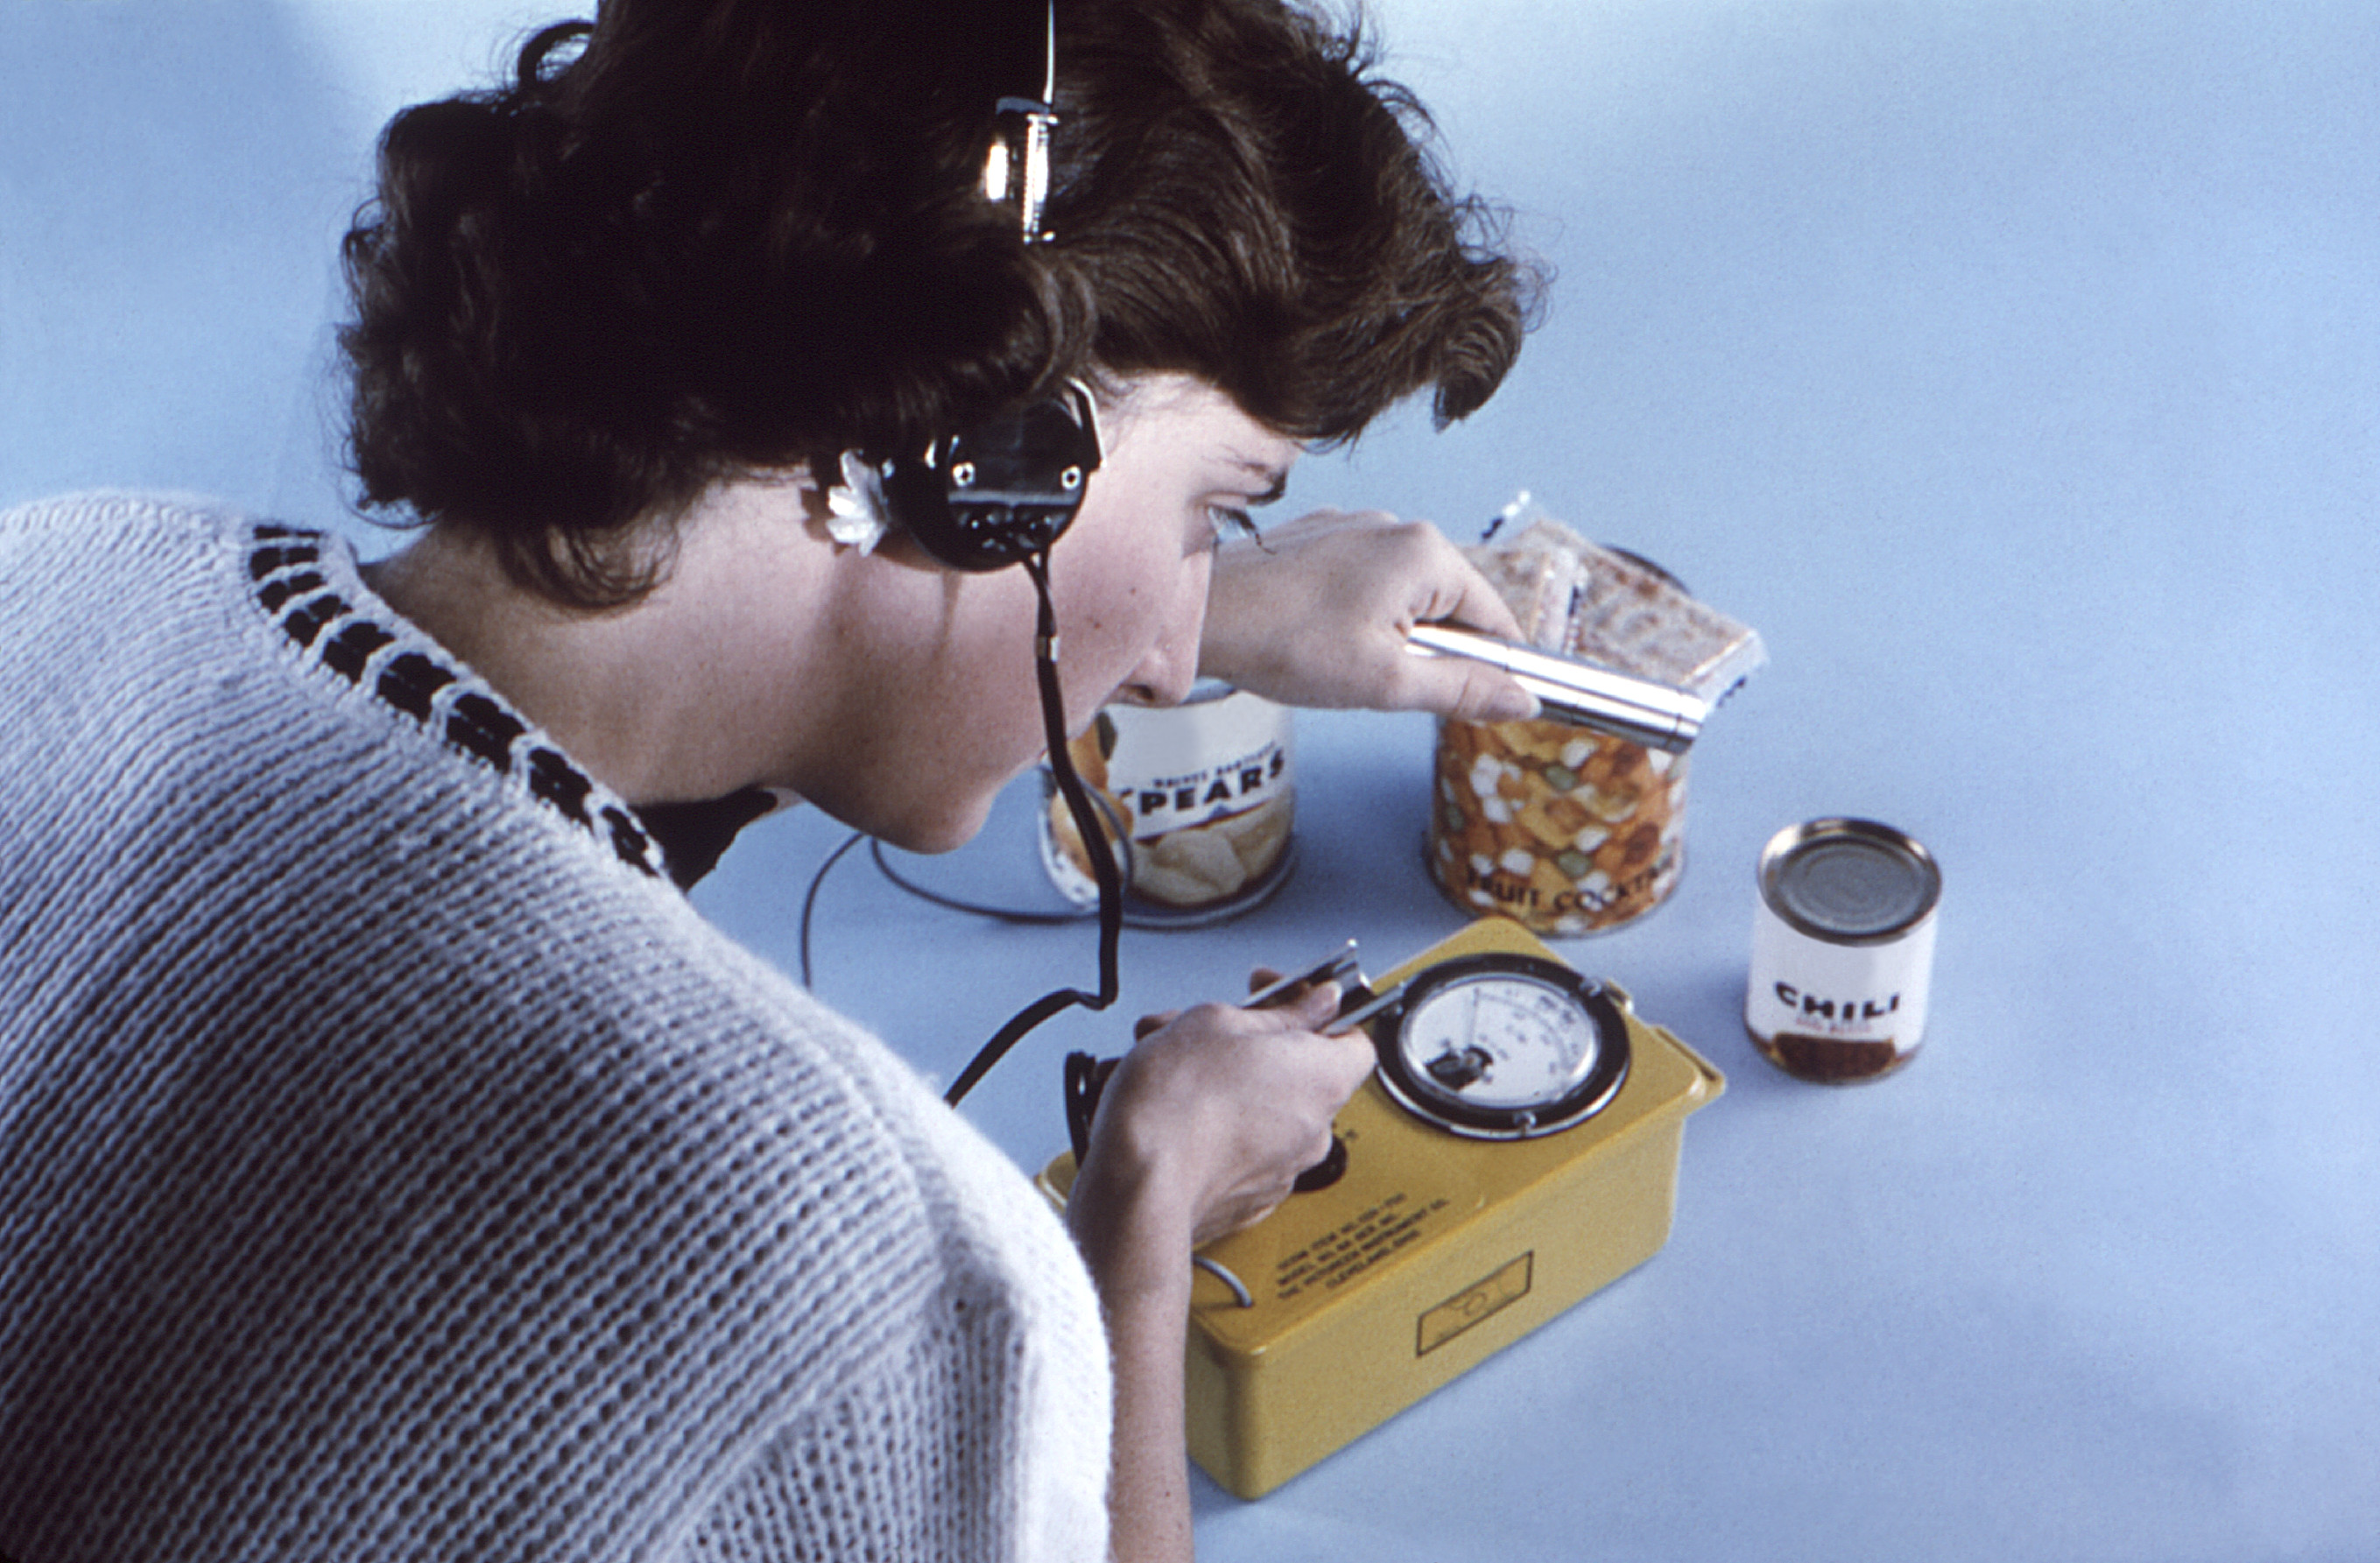
\includegraphics[width=1\linewidth]{figures/Geiger_counter_usage} 

}

\caption{Photograph depicting a Geiger counter being used to detect levels of radiation. Geiger counters use sonification to represent radioactivity by producing audible clicks that increase in frequency as the level of measured ionizing radiation increases \autocite{dobsonDetailsPublicHealth1963}.}\label{fig:geiger-counter}
\end{figure}

\hypertarget{monitoring-external-information}{%
\subsubsection{Monitoring external information}\label{monitoring-external-information}}

In a review of mapping strategies for sonification Dubus and Bresin \autocite{dubusSystematicReviewMapping2013} identify a number of applications for sonification, including monitoring, motion perception, data exploration, accessibility, art and aesthetics, complement to visualization and study of psychoacoustics. Debashi and Vickers \autocite{debashiSonificationNetworkTraffic2018} specify that sonification is a particularly useful tool for conveying the type of information that changes over time. Kramer et al. \autocite{kramerSonificationReportStatus1999} point out that sonification can allow the user to make sense of large amounts of data by utilizing modern powerful media technologies. Out of the various applications for sonification, monitoring of external information is the most relevant for the current study.

Using sonification for external monitoring can for example mean that there is a sound that the user listens to while simultaneously working on something else, such as when medical staff in operating rooms rely on auditory cues from their equipment to monitor the patient's vital signs \autocite{dubusInteractiveSonificationMotion2013}. In that type of situation a change to the monitored state causes a corresponding change in the sound, allowing the user to quickly become aware of the change and react as needed. One of the clear advantages with using sonification for external monitoring is then that the user is free to work on a different task than the monitoring while still maintaining the ability to detect and react to changes \autocite{vickersSonificationProcessMonitoring2011}.

Compared to visualization, sonification can have certain advantages that make it suitable as a complement or replacement to visualization. This can be observed in practice in the health sector, where real-time sonification using parameter mapping methods is used; one study identified a high potential and found positive results for the use of real-time auditory feedback-oriented training devices in physical rehabilitation and fitness training to increase awareness of physiological responses \autocite{yangRealtimeSonificationBiceps2015}. The fact that humans are very sensitive to changes in rhythm or sequences of sounds lends further support to the idea of complementing visualizations with sonification \autocite{hildebrandtShortPaperEnhancing2014}. A recent study by Debashi and Vickers \autocite{debashiSonificationNetworkTraffic2018} comparing sonification and visual methods of monitoring found that the visual method alone performed significantly worse than a combination of both, and further that using sonification resulted in reduced visual fatigue rates. In summary, the scientific literature clearly indicates that sonification has an important part to play in the context of monitoring external information, and furthermore its use cases extend to several different sectors and should be researched further.

\hypertarget{movement-sonification}{%
\subsubsection{Movement sonification}\label{movement-sonification}}

As previously mentioned, sonification involves the transformation of all types of data into sound \autocite{kramerSonificationReportStatus1999}. The term movement sonification specifically refers to the transformation of movement -- typically that of a human -- into sound \autocite{vinkenAuditoryCodingHuman2013}. \textcite{effenbergMovementSonificationEffects2005} states that perception and reproduction accuracy of gross motor patterns can be improved with the help of movement sonification, indicating a wide range of potential applications for artificial auditory movement information in sports and rehabilitation. Based on the idea that perceiving gross motor patterns is facilitated when more senses are active, Sport Scientist in particular have tried to take advantage of this effect by creating and conveying an increased amount of auditory movement information. In order to achieve multisensory integration benefits, it is vital that the additional auditory movement information corresponds to the structure of the perceptual features of another modality (visual, kinesthetic, or tactile) {[}gerdschmitzSoundJoinedActions2017{]}. When visual motion perception is the reference with which bi- or multimodal convergence is to be achieved, movement sonification needs to be based on kinematic parameters {[}gerdschmitzSoundJoinedActions2017{]}. These kinematic parameters refer to the spatiotemporal features of a movement pattern or pose. This acoustic enhancement of motor perception became known as ``movement sonification'' when \textcite{effenbergMovementSonificationEffects2005} took the sonification approach of the early 1990s and adapted it to the kinematics and dynamics of human motor actions.

In the empirical section of the current study, we describe how we used movement sonification to emphasize different joint action strategies and manipulate synchronization during a joint action task. The use of movement sonification in joint action research is supported by the finding that movement sonification enhances perception of movement and improves motor performance \autocite{schmitzObservationSonifiedMovements2013}. Other studies in Sport Science have found that when movements are mapped onto sound, i.e.~sonified, predictions can be facilitated {[}\textcite{effenbergMovementSonificationEffects2005}; schmitzPerceptualEffectsAuditory2012{]}. Movement sonification may also support synchronization in joint action by addressing central motor representations, more precisely by making the movements of athletes more predictable to their teammates \autocite{schmitzPerceptualEffectsAuditory2012}. Furthermore, sonification is well suited to support applications for physical training, as seen in a study by \textcite{dubusEvaluationFourModels2012} where professional rowers were able to use kinetic and kinematic cues to optimize their rowing speed. The author concluded that rowing performance could be improved with the help of interactive augmented feedback \autocite{dubusEvaluationFourModels2012}. Finally, \textcite{schmitzSoundJoinedActions2017} found that complementing visualizations of a swimmer with kinematic sonification allowed for more accurate perceptions of differences in swimming stroke frequency.

With sonification being such a recent field of research, its subfield movement sonification has had even less time to be researched \autocite{vinkenAuditoryCodingHuman2013}. As such, the question of how to map movement parameters onto sound in an optimal way remains uncertain due to a lack of an adequate theoretical background \autocite{effenbergAccelerationDecelerationConstant2018}. With this uncertainty in mind, \textcite{effenbergAccelerationDecelerationConstant2018} conclude that movement sonification can function as an accessible form of information similar to visual information when coded properly. Along the same lines, \textcite{vinkenAuditoryCodingHuman2013} also state that movement sonification can improve motor processes, as well as adding information to parts of movements that are typically silent. On the other hand, \textcite{vinkenAuditoryCodingHuman2013} explain that despite these potential use cases there is hardly any empirical data from scientific research that clarifies how to sonify gross motor human movement in order to achieve information rich sound sequences. For these reasons it is important to gather more data about both sonification in general, as well as movement sonification specifically.

\textcite{vinkenAuditoryCodingHuman2013} identify three main areas for movement sonification that are lacking in empirical proof: the selection of appropriate movement features, the optimal mapping patterns between kinetic and acoustic features, and the appropriate number of dimensions for sonification. The current study adds to the existing body of research in movement sonification by describing in detail, in the Methods section , our selection of movement and acoustic features, how they were mapped, and which dimensions were used. {[}Luke u may want to add something here{]}

Beyond just movement sonification, this study also furthers our understanding by investigating sonification in the context of learning a novel joint action task and improving performance of that task as measured by synchronization. Music belongs to the relatively small set of joint action behaviors that support a high degree of coordination, because of how suitable our auditory system is for temporal coordination \autocite{hildebrandtShortPaperEnhancing2014}. This raises the question of whether we can optimize temporal coordination by using movement sonification, and in short: can sonification help with joint action? The existing body of research falls short on this question, and the present study aims to open a discussion with the help of a pilot experiment conducted at Aarhus University. In the next section we will present the theory behind joint action with a focus on representations, action monitoring, and action prediction. Then, before presenting our pilot experiment, we will further discuss how and why the two concepts of sonification and joint action are integrated.

\hypertarget{joint-action}{%
\subsection{Joint action}\label{joint-action}}

Joint actions, where two or more people synchronize their actions in pursuit of a shared goal \autocite{knoblichPsychologicalResearchJoint2011}, are a regular part of human behavior. A longer definition refers to joint action as ``any form of social interaction whereby two or more individuals coordinate their actions in space and time to bring about a change in the environment'' \autocite[p.~1]{sebanzJointActionBodies2006}. With these definitions in mind, examples of joint action can include an extremely wide range of activities, such as handshakes, conversations, musical performances and partner dances, but also bank robberies and the building of the pyramids. To avoid overwhelming the reader, a typical example that is found in the literature \autocite{sebanzJointActionBodies2006} and that fits both definitions of joint action is when two people work together to carry a table from point A to point B.

As mentioned in the introduction, the progress of human civilization is largely based on working together. Joint actions constitute a significant part of the human experience, and they form an important and intriguing research topic for the field of cognitive science. Studies of joint actions such as putting together furniture or playing a piano duet, for instance, have shed light on how speech is used to establish who will do what and to agree on the details of the joint performance \autocite{clarkCoordinatingEachOther2005}. Additionally, research on how people solve problems of spatial coordination has shown that humans are capable of creating new symbol systems to coordinate their actions when conventional communication is not available \autocite{galantucciExperimentalSemioticsNew2009}.

Joint actions can be divided into two categories: emergent and planned coordination \autocite{knoblichPsychologicalResearchJoint2011}. Emergent coordination describes coordinated behavior arising from perception-action connections that lead to similar actions among individuals, independently of prior planning \autocite{knoblichPsychologicalResearchJoint2011}. An example of this is when pedestrians end up walking in step with each other without explicitly planning to do so. With regards to planned coordination, the behaviour of agents is driven by representations that describe the desired outcomes of joint action and the respective role of the agent in achieving these outcomes \autocite{knoblichPsychologicalResearchJoint2011}. Next we will describe the cognitive processes that are involved in the more relevant, planned coordination, category of joint action. In addition to representations, recent theory identifies action monitoring and action prediction as the other main cognitive processes involved in planned joint action {[}\textcite{loehrMonitoringIndividualJoint2013}; sebanzJointActionBodies2006; \textcite{vesperMinimalArchitectureJoint2010}{]}.

\hypertarget{representations}{%
\subsubsection{Representations}\label{representations}}

According to the minimal architecture for joint action proposed by \textcite{vesperMinimalArchitectureJoint2010}, an agent involved in joint action must, at a minimum, have a representation of their own task and the shared goal. An assumption is also that the shared goal cannot be achieved without the contribution of both parties \autocite{vesperMinimalArchitectureJoint2010}. In the model developed by \textcite{vesperMinimalArchitectureJoint2010}, the shared goal is expressed as ``ME + X'', where ``ME'' stands for the agent's own contribution, and ``X'' stands for the contribution that is not produced by the agent themselves. A study by \textcite{loehrSoundYouMe2016}, which had piano novices practice a duet with a more experienced pianist, found that the novices' representations consisted of the duet participants' shared goal, and to a small extent of the novices' own personal goal.

A minimal version of including the other in one's representations is theorized to be the understanding that the source of ``X'' -- that which is not produced by an agent themselves -- is the joint action partner {[}\textcite{loehrSoundYouMe2016}; vesperMinimalArchitectureJoint2010; Although it is not required, it is often helpful to also represent the other's task, as it allows for more precise predictions of what the other will do next {[}\textcite{boltSensoryAttenuationAuditory2021}; wenkeWhatSharedJoint2011{]}. As an example, consider two singers performing a duet together. Each singer must fully know their own part, while also representing the shared goal of synchronized singing. Although these two main representations can be sufficient for performing a duet, professional singers typically familiarize themselves with their singing partner's part in addition to their own, as it allows for a more polished and cohesive musical performance. The benefits of representing the other's task were demonstrated by a study \autocite{kellerPianistsDuetBetter2007} in which pianists were asked to record one part from a selection of piano duets and then play the complementary part in synchrony with either their own or other participants' recordings. The results showed that the pianists synchronized better with recordings of themselves than those of others, indicating that synchronization is facilitated by having a more precise representation of the auditory stimuli with which one is coordinating actions. Further insight into the role of representations in joint action comes from an EEG study by \textcite{kourtisPredictiveRepresentationOther2012}, which found that partners represented each other's actions in advance when passing an object, and doing so facilitated coordination. Having these shared representations of actions and their underlying goals allows individuals to establish a procedural common ground for joint action without needing to rely on symbolic communication \autocite{sebanzJointActionBodies2006}.

Two music-related studies have explored both shared and individual goals. First, @ kellerMusicalMeterAttention2005 demonstrated that musicians performing duets can attend to and recall both their own part and a combination of their own and a complementary part. More recently, \textcite{loehrMonitoringIndividualJoint2013} reported that duetting pianists prioritize shared goals (the musical harmony arising from both pianists' combined pitches) over individual action goals (the individual pitches played by each pianist), as demonstrated by stronger neural responses to pitch errors that impact the former compared to the latter. Based on their study, \textcite{loehrSoundYouMe2016} argue that shared goals are more salient compared to individual goals in novel joint actions performed by non-experts.

Empirical research of representations has largely focused on how people represent each individual's contributions to the joint action {[}\textcite{knoblichPsychologicalResearchJoint2011}; loehrSoundYouMe2016{]}. The details of how {[}cursive{]} people represent shared goals remain mostly unclear, however \autocite{loehrSoundYouMe2016}. Findings by \textcite{loehrSoundYouMe2016} indicate that novices in joint action contexts that promote minimal representations represent their actions in relation to the shared goal, which supports the argument that joint action participants represent the shared goal of the task \autocite{vesperMinimalArchitectureJoint2010}. Still, researchers highlight the need for further research, for instance by pointing out the lack of joint action studies teasing apart representations of shared and individual goals \autocite{loehrSoundYouMe2016}. The present study thus aims to fill this gap in joint action research by addressing both in the form of self-other- and joint outcome -strategies as separate experimental conditions.

\hypertarget{action-monitoring}{%
\subsubsection{Action monitoring}\label{action-monitoring}}

Another cognitive process involved in joint action is known as action monitoring, or simply monitoring. Representations, specifically shared task representations, are intrinsically linked with both monitoring and predicting processes, with all of them working together to enable interpersonal coordination in real time \autocite{knoblichPsychologicalResearchJoint2011}. \textcite{knoblichPsychologicalResearchJoint2011} describe this interplay of cognitive processes by stating that shared task representations determine how agents monitor and plan their actions. A simple way to consider this is that in order to effectively monitor an action, a basic idea of what it should resemble -- i.e., a task representation -- is required.

Monitoring processes are used to assess the extent to which a task or goal is being accomplished and whether actions are proceeding as intended \autocite{botvinickConflictMonitoringCognitive2001}. In terms of assessing task and goal progress, three things can be monitored: the agent's own task, the other's task, and the shared goal. The agent must at least monitor the progress of their own task and the shared goal. It is not strictly necessary to monitor the other's task, and it depends on the type of joint action that is performed. For example, consider a very simple task such as lifting an object straight up in the air together with a partner. It is entirely possible to do so successfully even if both agents only monitor their own task (``lift this side of the object'') and the shared goal (``lift this object together''). Nevertheless, it is likely true that monitoring what one's partner is doing will improve joint action performance -- especially for tasks that require precise synchronization \autocite{vesperMinimalArchitectureJoint2010}.

With respect to monitoring the sensory consequences or outcomes of joint actions, a distinction can be made between monitoring the individual outcomes vs joint outcomes. A study by \textcite{loehrMonitoringIndividualJoint2013} distinguished between individual and joint outcomes of actions with the help of a clever experiment, where experienced pianists played a pre-rehearsed duet on a digital piano while the outcomes of certain keypresses were manipulated by the researchers. In the individual outcome condition, the produced tones of keypresses were manipulated so that the harmony of the resulting chord remained the same. In the joint outcome condition, the produced tones were manipulated so that the harmony of the chord changed. The researchers found that the musicians in their study were able to monitor both individual and joint outcomes, while maintaining a distinction between the two. Furthermore, the musicians were able to monitor the outcomes of both their own and their partner's actions in parallel, while also differentiating between the two. To summarize, it appears that agents involved in joint action tend to represent and monitor their own and their partners' actions, as well as the joint outcome of their actions.

\hypertarget{action-prediction}{%
\subsubsection{Action prediction}\label{action-prediction}}

The crucial final feature of joint action relates to the manner in which individuals adapt their own actions to those of others in time and space, and doing so requires making predictions of the other's actions. In order to avoid constantly being one step behind during joint action, interacting partners cannot simply respond to observed actions, but must rather plan their own actions in relation to what they predict their partner will do \autocite{sebanzJointActionBodies2006}. This prediction process is achieved through motor simulation, which uses internal models to determine the sensory consequences of actions as well as their effect on the environment (Gerd Schmitz \& Alfred O. Effenberg, 2017; Vesper et al., 2010). Simulating the actions of others as they occur may be especially beneficial when engaging in joint action , and it has been suggested that such motor simulation influences perception and assists in predicting the consequences and timing of others' actions {[}vesperMinimalArchitectureJoint2010{]}. The idea that internal predictive models contribute to the ability to anticipate others' actions is supported by findings that short-term predictions of others' actions are based on one's own motor experience (Aglioti et al., 2008; Calvo-Merino et al., 2005){]}. The data from \textcite{loehrSoundYouMe2016} complement previous joint action research by strengthening the notion that agents can predict the consequences of others' actions in parallel with their own {[}\textcite{loehrMonitoringIndividualJoint2013}; vandersteenADaptationAnticipationModel2013; vesperOurActionsMy2014; wolpertUnifyingComputationalFramework2003{]} and also incorporate these predictions of other's actions when planning and executing their own actions {[}\textcite{knoblichActionCoordinationGroups2003}; kourtisPredictiveRepresentationOther2012; loehrTemporalCoordinationPerforming2011; vesperAreYouReady2013{]}.

It is not fully clear yet whether similar mechanisms exist specifically for predicting the joint outcome of an agent's and their partner's actions. Some support for predicting joint outcomes comes from a study by \textcite{knoblichActionCoordinationGroups2003}, which demonstrated the ability to predict combined outcomes through improved joint task performance with practice. The results showed that participants initially struggled with the joint task of controlling a cursor together to track a moving target on a computer screen, but with practice, performance reached the level of individual performance. Furthermore, participants who were provided with an external cue tone about the state of their partner's action were more successful at the task, indicating that auditory feedback can facilitate coordination \autocite{knoblichActionCoordinationGroups2003}. This is particularly interesting in the context of the present study, as it suggests a potential benefit with using sonification in the context of joint action.

\hypertarget{section-motivating-the-current-study}{%
\subsubsection{Section motivating the current study}\label{section-motivating-the-current-study}}

In this section, we will focus on how the concepts of sonification and joint action relate to each other. To briefly restate what has been previously discussed, sonification is defined as the transformation of data into sound \autocite{kramerSonificationReportStatus1999} and joint action refers to situations where two or more people synchronize their actions to achieve a shared goal \autocite{knoblichPsychologicalResearchJoint2011}. The cognitive processes related to joint action include representation, monitoring and prediction {[}\textcite{loehrMonitoringIndividualJoint2013}; sebanzJointActionBodies2006; \textcite{vesperMinimalArchitectureJoint2010}{]}. We will now discuss how sonification can make use of these three different processes in the light of previous research.

The first cognitive process in joint action to be considered is representation. There is no clear consensus in the academic literature on how an agent involved in joint action represents, but previous research indicates that the agent must, at the very least, represent their own task and the shared goal \autocite{vesperMinimalArchitectureJoint2010}. There are also several studies supporting the argument that representing the other's task can be beneficial for joint action by making prediction and synchronization easier {[}\textcite{boltSensoryAttenuationAuditory2021}; kellerPianistsDuetBetter2007; kourtisPredictiveRepresentationOther2012; sebanzJointActionBodies2006; wenkeWhatSharedJoint2011{]}. \textcite{loehrSoundYouMe2016} point out the need for future research to investigate which factors influence whether or not an agent represents their partner as the other source contributing to the shared goal, and how those representations of their partner may change while learning a joint action. In their study, \textcite{loehrSoundYouMe2016} found that novices have the ability to integrate the auditory effects of their partner's actions into their sensorimotor action representations while learning to play musical pieces together. The notion that such an ability is not limited only to experts is pertinent to the current study because it facilitates the exploration of learning novel joint action tasks using sonification. Specifically, sonification can be used to sonify an agent's own actions, their partner's actions, or the joint outcome of both participants. This allows us to direct participants' attention towards specific types of representations, namely self-other and joint outcome representations.

The next cognitive process to discuss in the context of joint action and sonification is monitoring. As stated earlier, a popular and useful application for sonification is the monitoring of external information \autocite{dubusSystematicReviewMapping2013}. Designing a sonification system for monitoring purposes requires careful consideration of various conditions and requirements. The sound must be capable of supporting extended periods of listening, changes in status have to be salient, and unexpected events have to be immediately apparent \autocite{kimotoDesignImplementationStetho2002}. In joint action, monitoring one's own actions and the progress towards the shared goal is crucial for success, and the other's actions must also be monitored when precise synchronization is required \autocite{vesperMinimalArchitectureJoint2010}. When discussing monitoring in joint actions, it is important to take into account the divided nature of joint action and identify the challenges that come with it. One of the main challenges arises from the fact that joint actions often require simultaneous actions by the participants, which may create the need for agents to monitor both their own and their partner's actions in parallel \autocite{loehrMonitoringIndividualJoint2013}. A closely related challenge is that monitoring an action, whether one's own or the other's, is dependent on having a representation of that action \autocite{knoblichPsychologicalResearchJoint2011}. The other main challenge relates to the fact that joint action outcomes are often more than the sum of individual action outcomes \autocite{loehrMonitoringIndividualJoint2013}. An example of this is how the same tones played by one musician can take on different qualities and become part of different harmonies, depending on what tones another musician is simultaneously playing \autocite{loehrMonitoringIndividualJoint2013}. This leads to the consideration of whether agents monitor their own or their partner's actions in relation to individual action goals (those required to achieve each individual's own task) or in relation to shared action goals (the joint outcome of their actions) \autocite{loehrMonitoringIndividualJoint2013}. In the current study, we attempt to address this challenge of individual vs joint outcomes by creating two different sonification schemes, where one scheme sonifies the individual action outcomes, and the other scheme sonifies the joint outcome of both participants' combined actions. We can therefore use sonification to encourage and facilitate monitoring of either individual (self-other) or joint outcomes. We theorize that the previously identified benefits of sonification in monitoring, such as the ability to work on another task while monitoring with one's ears \autocite{vickersSonificationProcessMonitoring2011} and the human auditory system's sensitivity to changes in sequences of sound \autocite{hildebrandtShortPaperEnhancing2014}, should improve performance of related joint action tasks by reducing the cognitive load required for monitoring. This reduction in cognitive load would then allow joint action participants to also focus on other points of interests that support progress towards the shared goal, such as fine motor control and planning their next actions. For these reasons, we postulate that sonification holds substantial promise for both practical applications and academic research of joint action monitoring.

The third and final cognitive process involved with joint action is prediction. Previous research in the field of Sport Science has revealed that sonification can improve perception accuracy of movements {[}\textcite{effenbergMovementSonificationEffects2005}; schmitzObservationSonifiedMovements2013{]}, revealing one potential mechanism by which predictions in joint action may be facilitated using sonification. As predictions play an important role in joint action \autocite{sebanzJointActionBodies2006} -- especially for tasks that require a high degree of synchronization {[}\textcite{vesperMinimalArchitectureJoint2010} -- we suggest that joint action performance can be improved by facilitating action prediction with the use of sonification. This is substantiated by the findings of \textcite{knoblichActionCoordinationGroups2003}, which revealed that joint action performance in a task requiring participants to predict joint outcomes improved when participants were provided with an external cue tone relating to their partner's actions. Further research needs to be conducted in order to determine whether auditory cues using sonification can facilitate prediction in other joint action contexts, and the present study aims to contribute to this body of research by using a joint action task that emulates the need for a high degree of synchronization.

Some of the questions that have been investigated in recent joint action research concern the aforementioned cognitive processes (representations, action monitoring and action predicting) and how they relate to agency (self vs other) and outcome (individual vs joint). Researchers have studied whether agents involved in joint action represent both their own task and their partner's task \autocite{loehrSoundYouMe2016}, whether they monitor individual outcomes or joint outcomes {[}loehrMonitoringIndividualJoint2013{]}, and how predictions of other's actions are incorporated when planning and executing actions {[}\textcite{knoblichActionCoordinationGroups2003}; kourtisPredictiveRepresentationOther2012; loehrTemporalCoordinationPerforming2011; vesperAreYouReady2013{]}. Based on the literature, a common denominator between sonification and joint action seems to be synchronization. For this reason, we identify a potential application for sonification particularly in joint action tasks that require a high degree of synchronization. Previous research has found that sonification can improve synchronization in joint action by addressing central motor representations \autocite{schmitzPerceptualEffectsAuditory2012} and monitoring \autocite{vesperMinimalArchitectureJoint2010}. More generally, several authors have argued that having more precise representations may be key to improving synchronization in joint action {[}\textcite{boltSensoryAttenuationAuditory2021}; kellerPianistsDuetBetter2007; kourtisPredictiveRepresentationOther2012; sebanzJointActionBodies2006; wenkeWhatSharedJoint2011. Sonification also appears to be useful for sensori-motor learning by providing auditory feedback of movements \autocite{bevilacquaSensoriMotorLearningMovement2016} and in the present study we address this aspect by giving subjects a novel joint action task with varying methods of auditory feedback.

In summary, this study adds to the discussion about strategies relating to joint action representations, namely self-other and joint outcome representations, by investigating their potential effect on synchronization. Participants in our study performed a novel joint action task under three different conditions -- individual outcome, joint outcome, and a control condition -- where the sensory consequences were manipulated through real-time sonification of movement. The sonification was used to prime the participants' attention towards either individual or joint, while joint task synchronization was recorded.

\hypertarget{research-question}{%
\subsubsection{Research question}\label{research-question}}

Is synchrony optimized when focusing on self-other representations or joint outcome representations?

\hypertarget{low-latency-motion-capture-sonification-validation-experiment}{%
\section{Low Latency Motion Capture Sonification Validation Experiment}\label{low-latency-motion-capture-sonification-validation-experiment}}

A pilot experiment was conducted to assess the viability of the sonification framework in a laboratory setting. This experiment required blindfolded subjects to move their assigned sleds along parallel tracks and use sounds they hear to remain as spatially synchronized on their tracks as possible.

\hypertarget{participants}{%
\subsection{Participants}\label{participants}}

An availability sample of ten subjects (age range 20-29 years; 5 female, 4 male, 1 gender-fluid; 7 right-handed, 2 left-handed, 1 ambidextrous) were recruited to participate in pairs. Subjects optionally reported basic demographic information regarding age range (intervals of 10, i.e.~10-19, 20-29, \ldots, 90-99), gender, handedness, years of formal music training and reported if they were known to be tone-deaf (6 not tone-deaf, 4 unknown). Subjects reported a mean of 2.4 years of formal music training (SD=4.2; min=0.0; max = 12.0 years). Due to this experiment being a pilot, five subject pairs were regarded as sufficient to validate the experimental setup as well as gather preliminary data on movement synchronization for the three conditions. Additionally, the number of possible participants were constrained by limited access to the motion capture system laboratory, which is shared by other researchers, meaning that subjects needed to be available at the scheduled lab times within the study timeframe.

\hypertarget{track-and-sleds}{%
\subsection{Track and Sleds}\label{track-and-sleds}}

Two parallel tracks were designed with a sigmoid curve shape, surfaced with a smooth veneer that allowed for free movement along the length of the track. Two identical sleds made from LEGO parts were constructed and three felt adhesive pads were attached to the underside of each to reduce resistance during movement. The sleds were coated with a matte black paint to limit near-infrared reflectivity \autocite{benedictSurveyMaterialsCoatings2016}, as prior tests with unpainted LEGO bricks introduced artifacts into the motion capture system that were incorrectly identified as markers.

\hypertarget{frequency-range-selection}{%
\subsection{Frequency Range Selection}\label{frequency-range-selection}}

Two distinct, continuous frequency ranges were selected for application in sonification conditions. These ranges are offset by a perfect fifth and span eight semitones. The overtone (the tone with the higher frequency) range was chosen based on a center frequency of 220 Hz (A3) and the range was limited to avoid a large overlap with the undertone (the tone with the lower frequency) range during normal operation (Table \ref{tab:frequency-ranges}). Consideration was also given to creating ranges that were not sufficiently high to cause discomfort at a consistent amplitude. \textcite{setharesSoundSound2005} show that perceived dissonance between two tones varies by the lower tone's frequency indicating that the selected undertone range of approximately 116 -- 227 Hz would increase in sensory dissonance as the distance between the two frequencies decreases and at a fifth interval, the two tones would be perceived as more consonant.

\begin{table}[!h]

\begin{threeparttable}
\caption{\label{tab:frequency-ranges}Frequency ranges for the two tones used in the sonification conditions. Note names are in International Pitch Notation, and are the closest approximation. Overtone frequencies were calculated to have a center frequency of 440Hz, and undertone frequencies are two-thirds of their overtone counterparts.}
\centering
\fontsize{7}{9}\selectfont
\begin{tabular}[t]{>{}l>{}l>{}r>{}c>{}r>{}c>{}r}
\toprule
\multicolumn{1}{c}{} & \multicolumn{2}{c}{Lower Bound} & \multicolumn{2}{c}{Center} & \multicolumn{2}{c}{Upper Bound} \\
\cmidrule(l{3pt}r{3pt}){2-3} \cmidrule(l{3pt}r{3pt}){4-5} \cmidrule(l{3pt}r{3pt}){6-7}
  & Freq & Note\textsuperscript{a} & Freq & Note\textsuperscript{a} & Freq & Note\textsuperscript{a}\\
\midrule
Overtone & 175 & F3 & 220 & A3 & 277 & C\#4\\
Undertone & 116 & A\#2 & 147 & D3 & 185 & F\#3\\
\bottomrule
\end{tabular}
\begin{tablenotes}
\small
\item [] 
\rightskip2em
{\footnotesize \sffamily \textsuperscript{a}Note names are in International Pitch Notation, and are the closest approximation to the frequencies used}
\item [] 
\rightskip2em
{\footnotesize \sffamily \textit{Note.} Overtone frequencies were calculated to have a center frequency of 440Hz, and undertone frequencies are two-thirds of their overtone counterparts.}
\end{tablenotes}
\end{threeparttable}
\end{table}



\begin{figure}[h]

{\centering 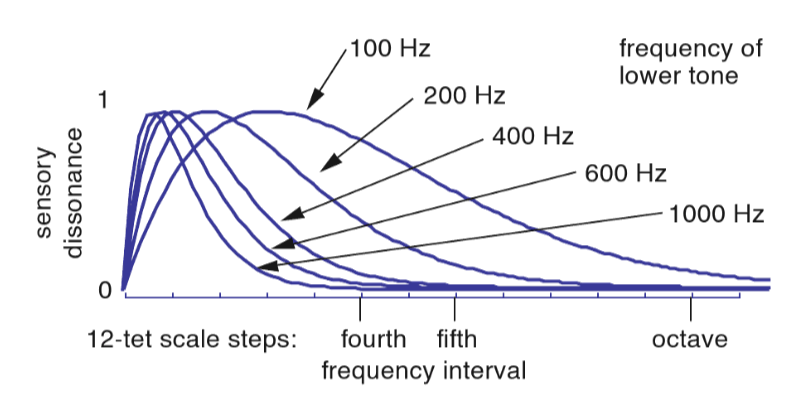
\includegraphics[width=1\linewidth]{figures/setharesTuningTimbreSpectrum2010_p47} 

}

\caption{Sensory dissonance of sine waves by interval for five frequencies. Figure \autocite[p.~47]{setharesSoundSound2005}}\label{fig:sensory-dissonance}
\end{figure}

\hypertarget{task-and-procedure}{%
\section{Task and Procedure}\label{task-and-procedure}}

Participants were asked to sit on opposite sides of the track structure and familiarize themselves with the movement of the sleds along the tracks. They were instructed to continuously move the sleds along the track from end to end, as rapidly as possible while remaining spatially synchronized with their partner's position on their respective track, using sounds they may hear during the various conditions to assist them. Once the participants had given their informed consent and been briefed, they would indicate when they were ready and were blindfolded for the duration of all trials within a condition. The experiment flow control was automated, starting with a practice trial of 30 seconds then a 15 second break followed by three experimental trials running for 90 seconds each with 15 second breaks between trials. Three tones played immediately prior to each trial to indicate the start of the trial, and a single tone played at the end of the trial to indicate the completion and participants were asked to return their sleds to the start of the track. Sonification and recording were paused between conditions to allow sufficient time for subjects to rest and answer the IOS survey. When the subjects were ready, a hardware button on the Bela was pressed to begin the next condition.

(prioritized comfort, allowed choice of arm despite handedness) {[}why this many, why not more, etc, ethics{]} Subjects were given and signed an informed consent form {[}appendix\ldots{]} and information sheet {[}appendix\ldots{]}\ldots{} and were under the umbrella project\ldots{}

\hypertarget{sonification-strategy-conditions}{%
\subsection{Sonification Strategy Conditions}\label{sonification-strategy-conditions}}

The experiment consisted of three conditions that vary the sonification strategy employed, namely: a no sonification control condition, a task-oriented sonification strategy and a synchronization-oriented sonification strategy. Each condition consisted of one practice trial of 30 seconds duration, and three main trials of 90 seconds each. Before each practice trial, subjects were reminded that it was a shorter trial and that they may use it to experiment with the sonification.

\hypertarget{no-sonification}{%
\subsubsection{No sonification}\label{no-sonification}}

In the no sonification condition, only the motion capture data from participants' sleds were recorded, and subjects could use the audible sounds of the sleds moving along the track to align themselves with their partner.

\hypertarget{task-oriented-sonification-strategy}{%
\subsubsection{Task-oriented sonification strategy}\label{task-oriented-sonification-strategy}}

Task oriented sonification represented the position of each sled along the length of the track as a synthesized tone that varied in frequency from highest to lowest at the start and end of the track respectively. One sled produced a higher frequency overtone, while the other produced a lower frequency undertone. If subjects were at the exact same x-coordinate, the two tones would be a perfect fifth apart, creating a harmonious chord, as the sleds drift further apart, the frequency difference would deviate from the perfect fifth and create a more discordant sound, Figure \ref{fig:task-illustration} illustrates the implementation of the task-oriented sonification strategy. This strategy was selected for sonifying the movement along the track, i.e.~the task required of subjects .

\begin{figure}[h]

{\centering 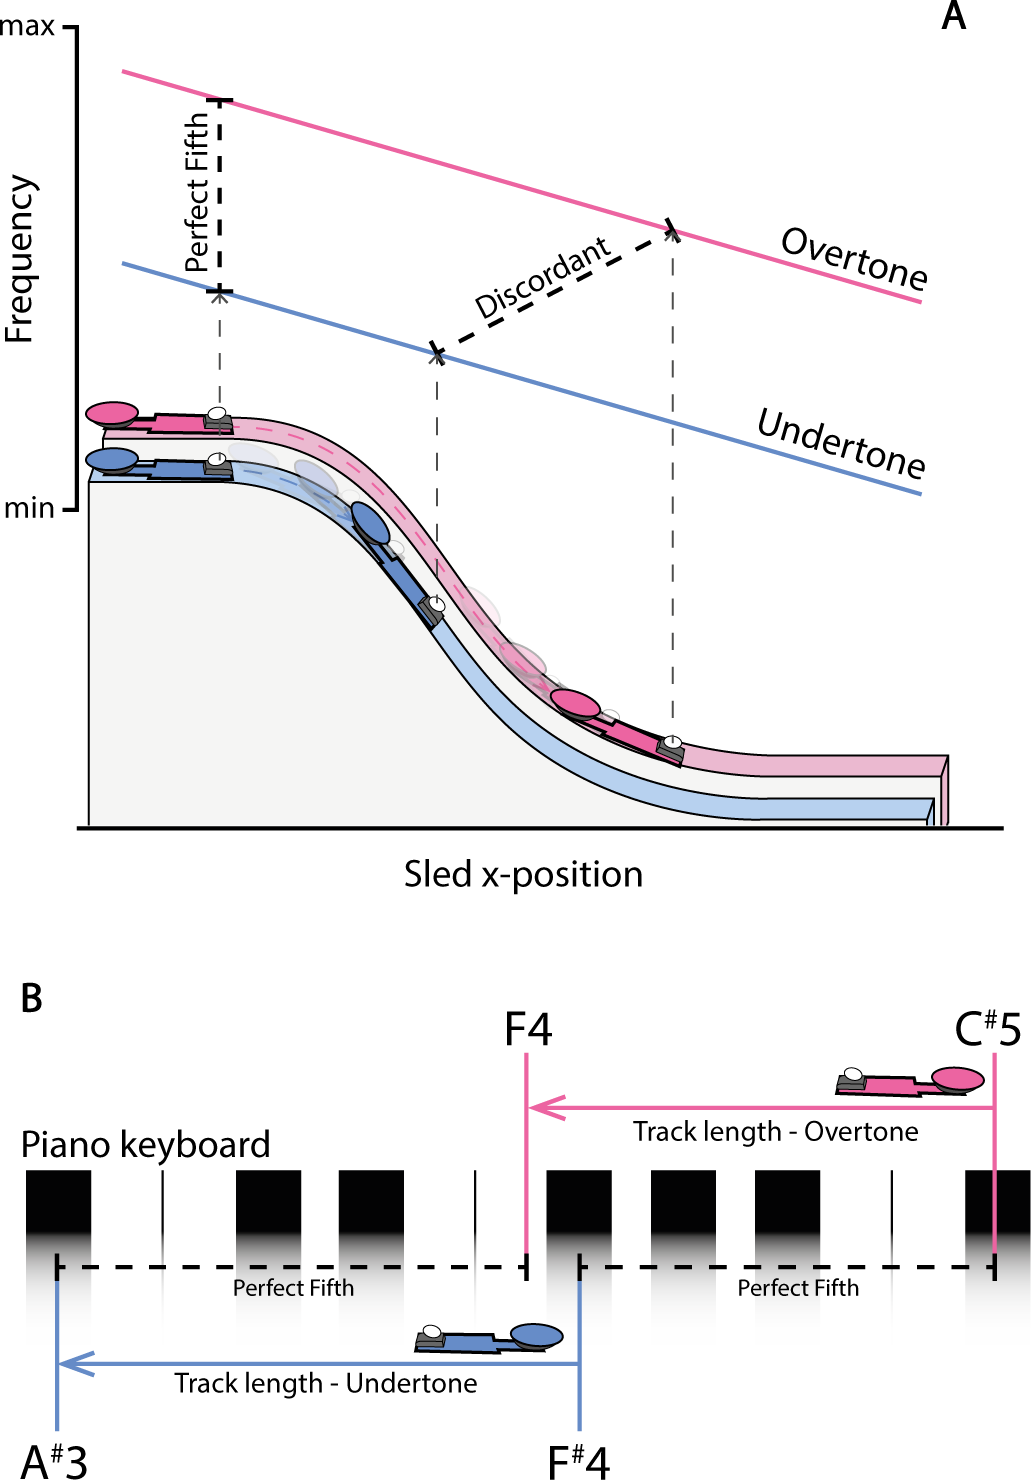
\includegraphics[width=1\linewidth]{figures/task_sonif_illustration} 

}

\caption{Task}\label{fig:task-illustration}
\end{figure}

\hypertarget{synchronization-oriented-sonification-strategy}{%
\subsubsection{Synchronization-oriented sonification strategy}\label{synchronization-oriented-sonification-strategy}}

The sonification strategy oriented around synchronization represented the position of the sleds relative to each other, where subjects with sleds at the same x-coordinates would hear a harmonious perfect fifth chord. When sleds would drift apart, the overtone amplitude would decrease, and the undertone frequency would change based on the distance between the two sleds, Figure \ref{fig:sync-illustration} illustrates the implementation of the synchronization-oriented sonification strategy.

\begin{figure}[h]

{\centering 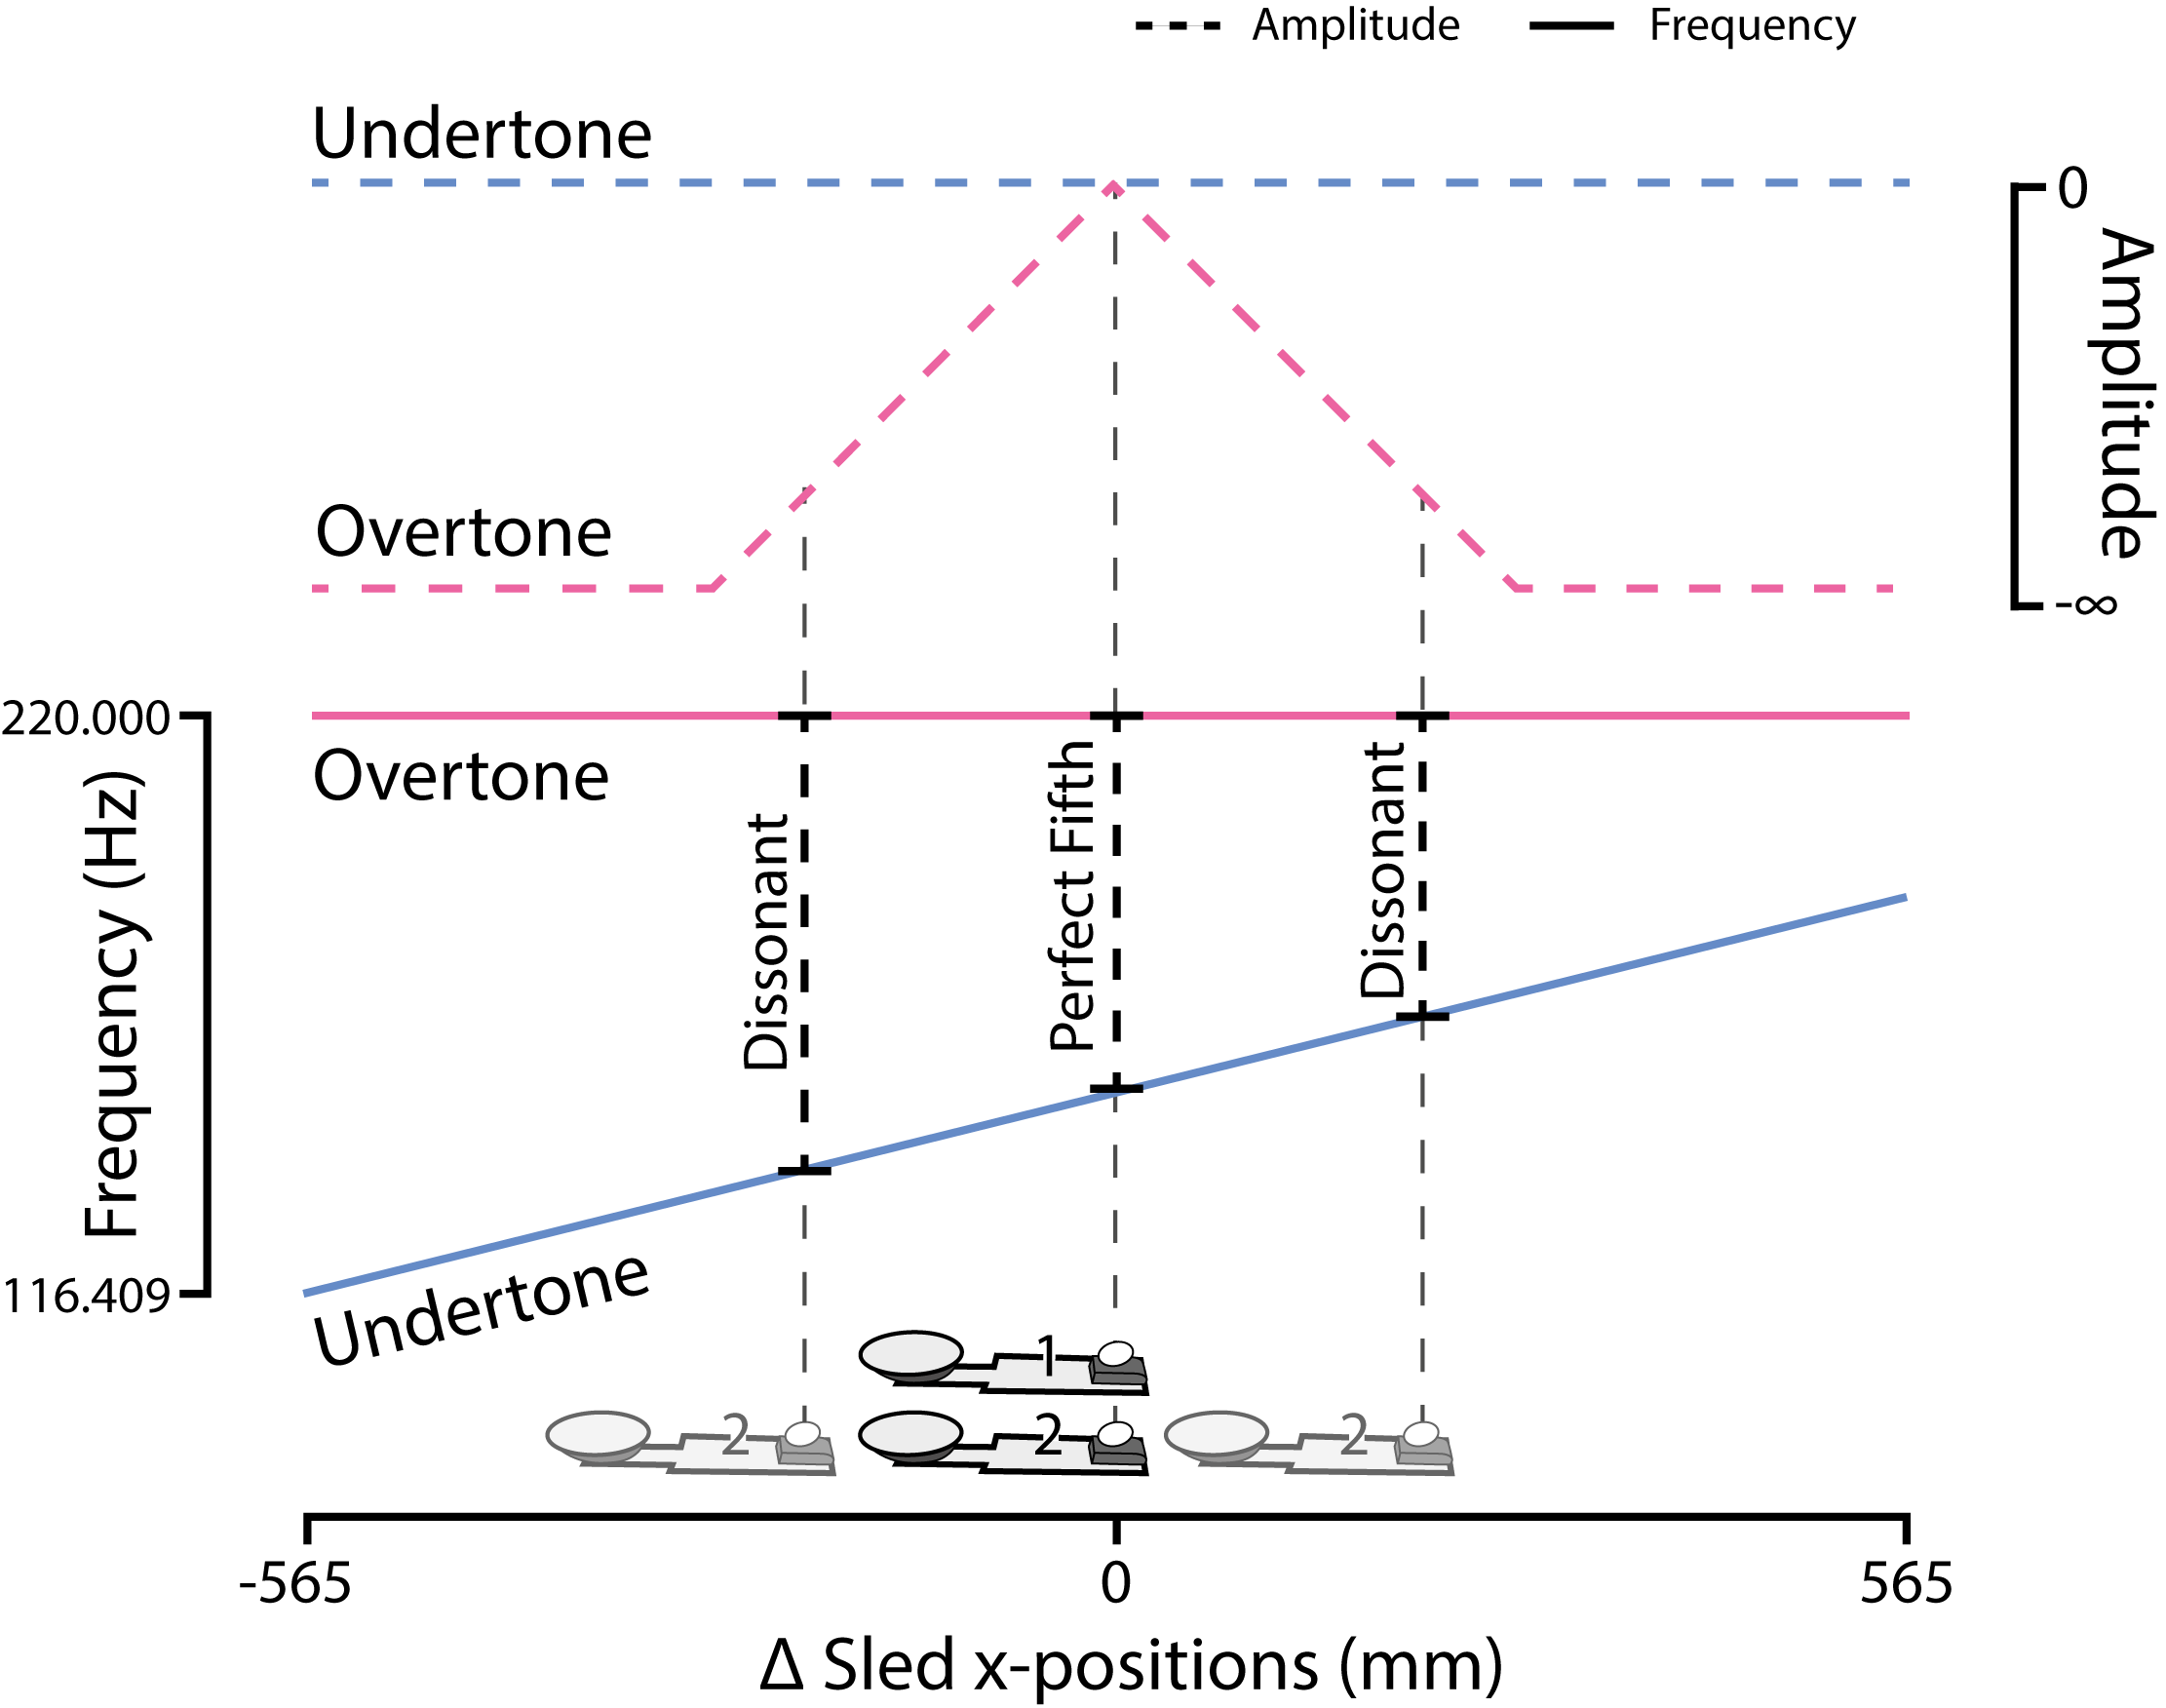
\includegraphics[width=1\linewidth]{figures/sync_sonif_illustration} 

}

\caption{Sync}\label{fig:sync-illustration}
\end{figure}

\hypertarget{hardware-and-software-implementation}{%
\section{Hardware and Software Implementation}\label{hardware-and-software-implementation}}

\hypertarget{motion-capture}{%
\subsection{Motion Capture}\label{motion-capture}}

Motion capture data were collected using a 9 camera (8 Qualisys Miqus M3 marker and 1 Qualisys Miqus Video) system connected to a Qualisys Camera Sync Unit. Marker data were acquired at a sampling rate of 300 Hz and video data were acquired at a sampling rate of 25 Hz. Qualisys Track Manager (QTM) software version 2022.2 (build 7700) was used to collect and process the data with real-time 3D tracking data output. QTM options for `processing of every frame' and `2D data preprocessing' were disabled for real-time output to ensure minimal latency. Figure \ref{fig:exp-graph} outlines the flow of data from motion capture to sonification.

\begin{figure}[h]

{\centering 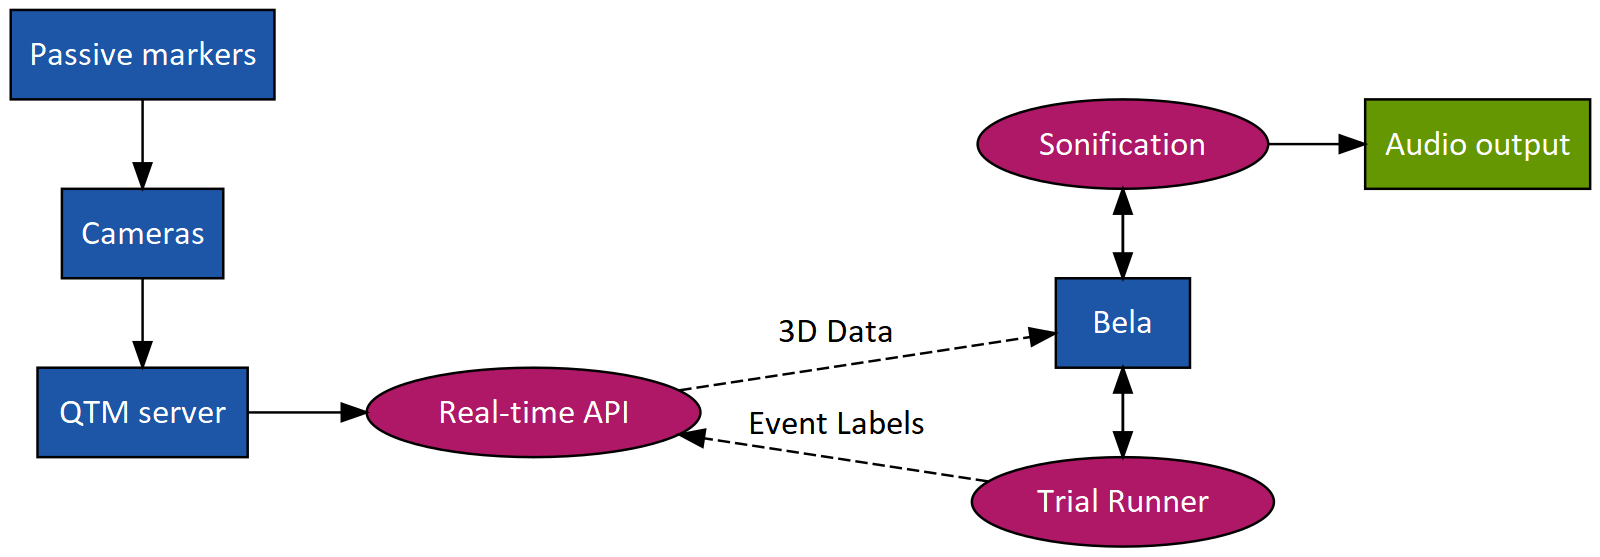
\includegraphics[width=1\linewidth]{figures/exp-graph} 

}

\caption{Low-latency sonification pipeline}\label{fig:exp-graph}
\end{figure}

\hypertarget{markers}{%
\subsubsection{Markers}\label{markers}}

For the experimental set up, one passive marker was placed on each car, and two additional passive reference markers were placed on the front corners of the track (see Figure \ref{fig:track-setup} for a visual representation of the track and marker placement). These additional markers provided reference points for 3D orientation of the track and the cars across trials in case of accidental track movement. Four preliminary sessions of two minutes were recorded of variable speed sled movements in QTM, and unique labels were given to the four passive markers. The recordings were used for training a QTM Automatic Identification of Marker (AIM) model. AIM models were applied to recordings and real-time output to apply known labels to marker data, allowing the sonification to read the current position of both sleds.

\begin{figure}[h]

{\centering 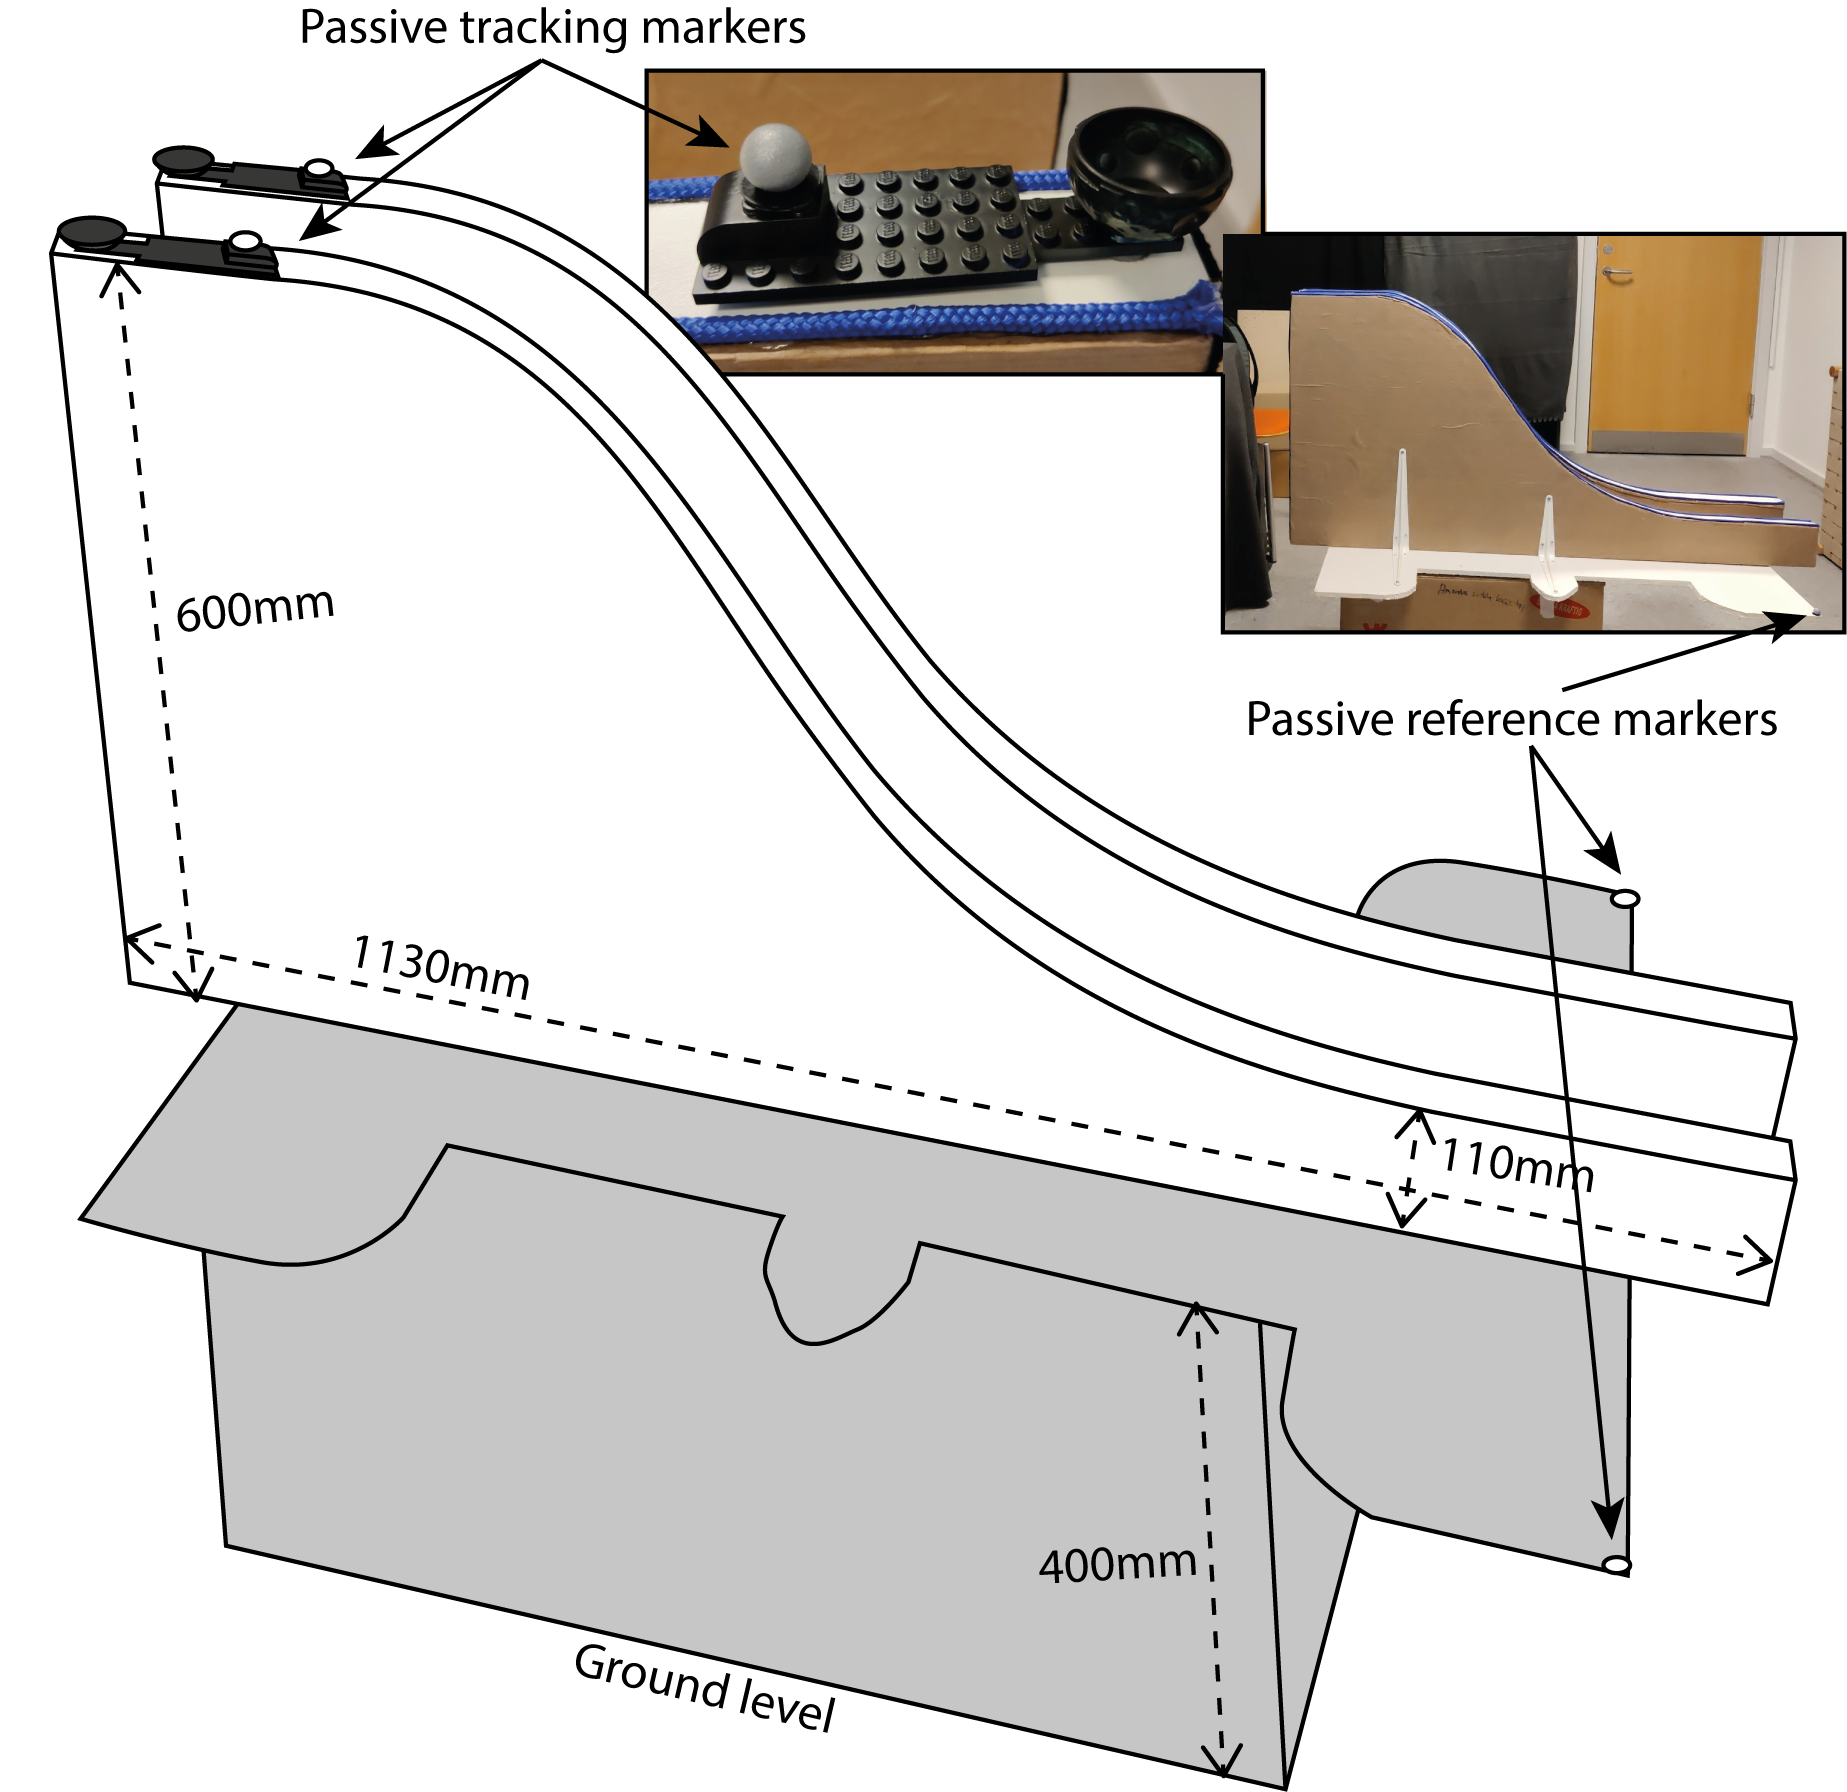
\includegraphics[width=1\linewidth]{figures/track_dimensions} 

}

\caption{Illustration depicting the experimental track setup and dimensions. Photos depict the constructed track as well as the sleds with the passive motion tracking markers.}\label{fig:track-setup}
\end{figure}

\hypertarget{sonification-1}{%
\subsection{Sonification}\label{sonification-1}}

Motion capture data were sent via UDP packets over USB networking to a Bela Mini device running version 0.3.8g running a custom C++ program\footnote{Source, data and analyses are available at \url{https://github.com/zeyus/QTM_Bela_Sonification}}. The main program loop was configured to execute every 32 samples, with an output sample rate of \ensuremath{4.41\times 10^{4}} Hz for 2 audio channels. The two audio output channels were connected to a pair of Genelec G Two active speakers. The main program used the latest available Bela platform framework \footnote{Commit ID \texttt{42bbf18c3710ed82cdf24b09ab72ac2239bf148e} from 10 August 2022: \url{https://github.com/BelaPlatform/Bela/commit/42bbf18c3710ed82cdf24b09ab72ac2239bf148e}}.

Two 16-bit 44.1 kHz wave files were prepared from the output of a MIDI synthesizer at the lowest frequency for both of the tones, and were cut off at 113145 samples where the zero-crossing of both files aligned. A 5ms fade-in and fade-out was applied to the start and end of the files to minimize DC pop. To allow for dynamic frequency changes, sound file playback used a floating point read pointer which was incremented sequentially as the 32ms buffer was populated. When the playback frequency was increased, the step size of the read position would increase by change in frequency, and would proportionally interpolate between samples to provide a smooth sounding frequency transition. This method was selected to ensure that the audio resolution was never below the original file's resolution.

\hypertarget{real-time-3d-data}{%
\subsubsection{Real-time 3D Data}\label{real-time-3d-data}}

A version of the Qualisys C++ SDK using protocol version 1.23 was modified to be compatible with the Bela platform and was used for communicating with QTM. To reduce latency, connection to the QTM server was made over UDP, and round-trip communication latency was verified by performing 1000 requests to the QTM server and logging the elapsed round-trip time, resulting in a mean latency of 0.25ms (SD 0.03ms, min 0.23ms, max 0.43ms).

Using the SDK, 3D streaming was initiated at the start of each sonification condition, and labelled markers were used to obtain the current position of each sled. The coordinates of the sleds were stored in a buffer containing the current and last recorded coordinates.

\hypertarget{experiment}{%
\subsection{Experiment}\label{experiment}}

\hypertarget{workflow}{%
\subsubsection{Workflow}\label{workflow}}

The experiment flow control was automated via the main C++ application running on the Bela mini. Before each experiment started, the condition order was configured in the application, and after compilation the suite of conditions and trials would run. Prior to commencement of each condition, the execution of the application halted to allow sufficient time for subjects to rest and to answer the IOS survey between conditions, after which a hardware button on the Bela could be pressed to continue. After commencement of a condition, all trials for that condition were run consecutively with 15 second breaks between them.

\hypertarget{event-labels}{%
\subsubsection{Event Labels}\label{event-labels}}

From the main Bela application, event labels indicating the start of an experiment suite, start and end of a condition and the start and end of individual trials were sent to the QTM server. These labels appear in the recorded 3D data and were exported alongside the marker positions for use in analysis and enable data to be segmented into their respective conditions and trials.

\hypertarget{analyses}{%
\section{Analyses}\label{analyses}}

General timing stuff, project specific stuff.

\hypertarget{data-preprocessing}{%
\subsection{Data Preprocessing}\label{data-preprocessing}}

\hypertarget{qtm}{%
\subsubsection{QTM}\label{qtm}}

Each session recorded had the AIM model applied to the duration of the recording, and labelled markers were manually verified and adjusted as required to ensure that for each completed trial, there was 100\% coverage of the marker data.

\hypertarget{d-data}{%
\subsubsection{3D Data}\label{d-data}}

3D data were exported from QTM and several preprocessing scripts were developed using the R programming language. Data were imported and collated by unique subject pair, condition and trial using the indices of the associated event labels, subsequently, practice trials, data outside of trials and invalid trials were removed. Invalid trials were defined as trials that did not have both a start and end event label. Trajectories were then created from marker x-coordinate time series using the R package \texttt{mousetrap} \autocite{mousetrap2021} which was designed to aid analyses of mouse movement trajectories, and is able to be applied to arbitrary spatial data. The starting position of trajectories were aligned to account for track movement between trials as well as axis misalignment, and x-axis trajectories were standardized within trials to have a mean of zero and a range from -1 to 1 allowing comparison between subject pairs, conditions and trials. Visual inspection of trajectory data was performed, and six trials where participants had lost control of the sleds were truncated to the time of the incident. This left a total of 44 experimental trials (38 complete and 6 truncated, partial trials), meaning observation data were available for all subject pairs in all conditions, with a single trial unavailable for the no sonification condition from one subject pair.

\hypertarget{subject-synchronization}{%
\subsection{Subject Synchronization}\label{subject-synchronization}}

Three methods were used on data collected from the expeirment to assess the level of synchrony between the participants in the various sonification conditions. The first method, absolute spatial distance (delta), provides a simple and straightforward measure of the overall synchrony between the sleds, but does not account for the temporal dynamics of the movement. The second method, Instantaneous Phase Angle Difference, provides real-time information about the synchrony of the movement, but may be sensitive to noise in the data and requires a good understanding of the mathematics involved. The third method, Dynamic Time Warping, offers a detailed analysis of the temporal dynamics of the movement and can handle differences in the speed of the movement, but may be computationally intensive and sensitive to the choice of the time-warping parameter. Each of the three methods has its own strengths and limitations, and the choice of which method to use will depend on the specific goals and requirements of the analysis.

\hypertarget{absolute-spatial-distance}{%
\subsubsection{Absolute Spatial Distance}\label{absolute-spatial-distance}}

Distance between subject sleds is a useful proxy for determining the level of success of synchronization, where a trial where subjects move perfectly together would result in a delta of zero for each time point, and large distances would indicate that they were unable to synchronize their sled movements. Absolute distance deltas between the standardized x-coordinates of subject pairs were calculated for each time point by trial and condition. Mean deltas per condition were calculated per subject pair, resulting in\ldots.. (Figure \ref{fig:pairwise-position-delta}). The distance delta alone is a crude measurement, and is unable to describe more complex interactions over time such as the leader-follower dynamics and changes in acceleration.
Table\ldots{}

\begin{figure}[h]

{\centering 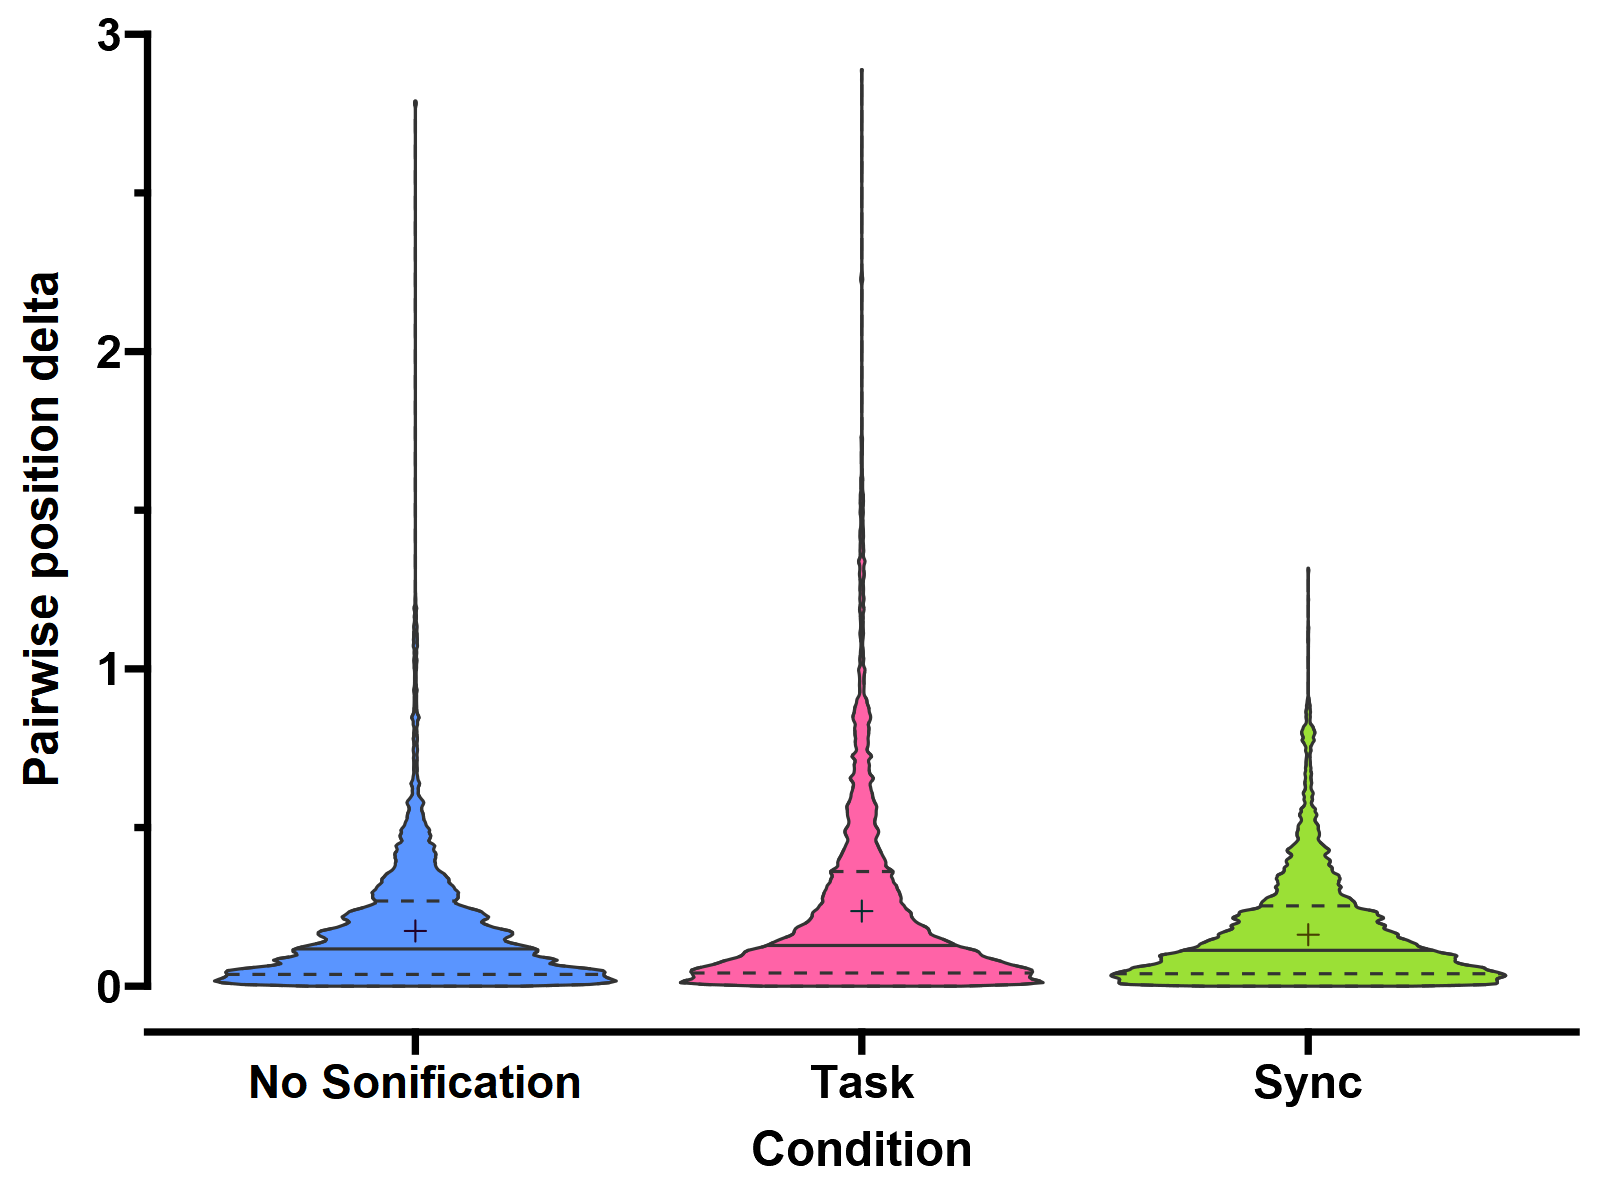
\includegraphics[width=1\linewidth]{figures/parwise_position_delta} 

}

\caption{Plot of pairwise position delta for each subject pair}\label{fig:pairwise-position-delta}
\end{figure}

\hypertarget{instantaneous-phase-angle-of-trajectories}{%
\subsubsection{Instantaneous Phase Angle of Trajectories}\label{instantaneous-phase-angle-of-trajectories}}

Instantaneous phase angles provide a way to determine differences in position, acceleration\ldots{}
The trajectory data were processed using a Hilbert transform, which resulted in the calculation of the instantaneous phase angle for each subject at each time point. The angle difference between subject pairs were calculated for each time point and the absolute difference in instantaneous phase angles were used to determine the mean angle difference and standard deviation for each condition.

\begin{figure}[h]

{\centering 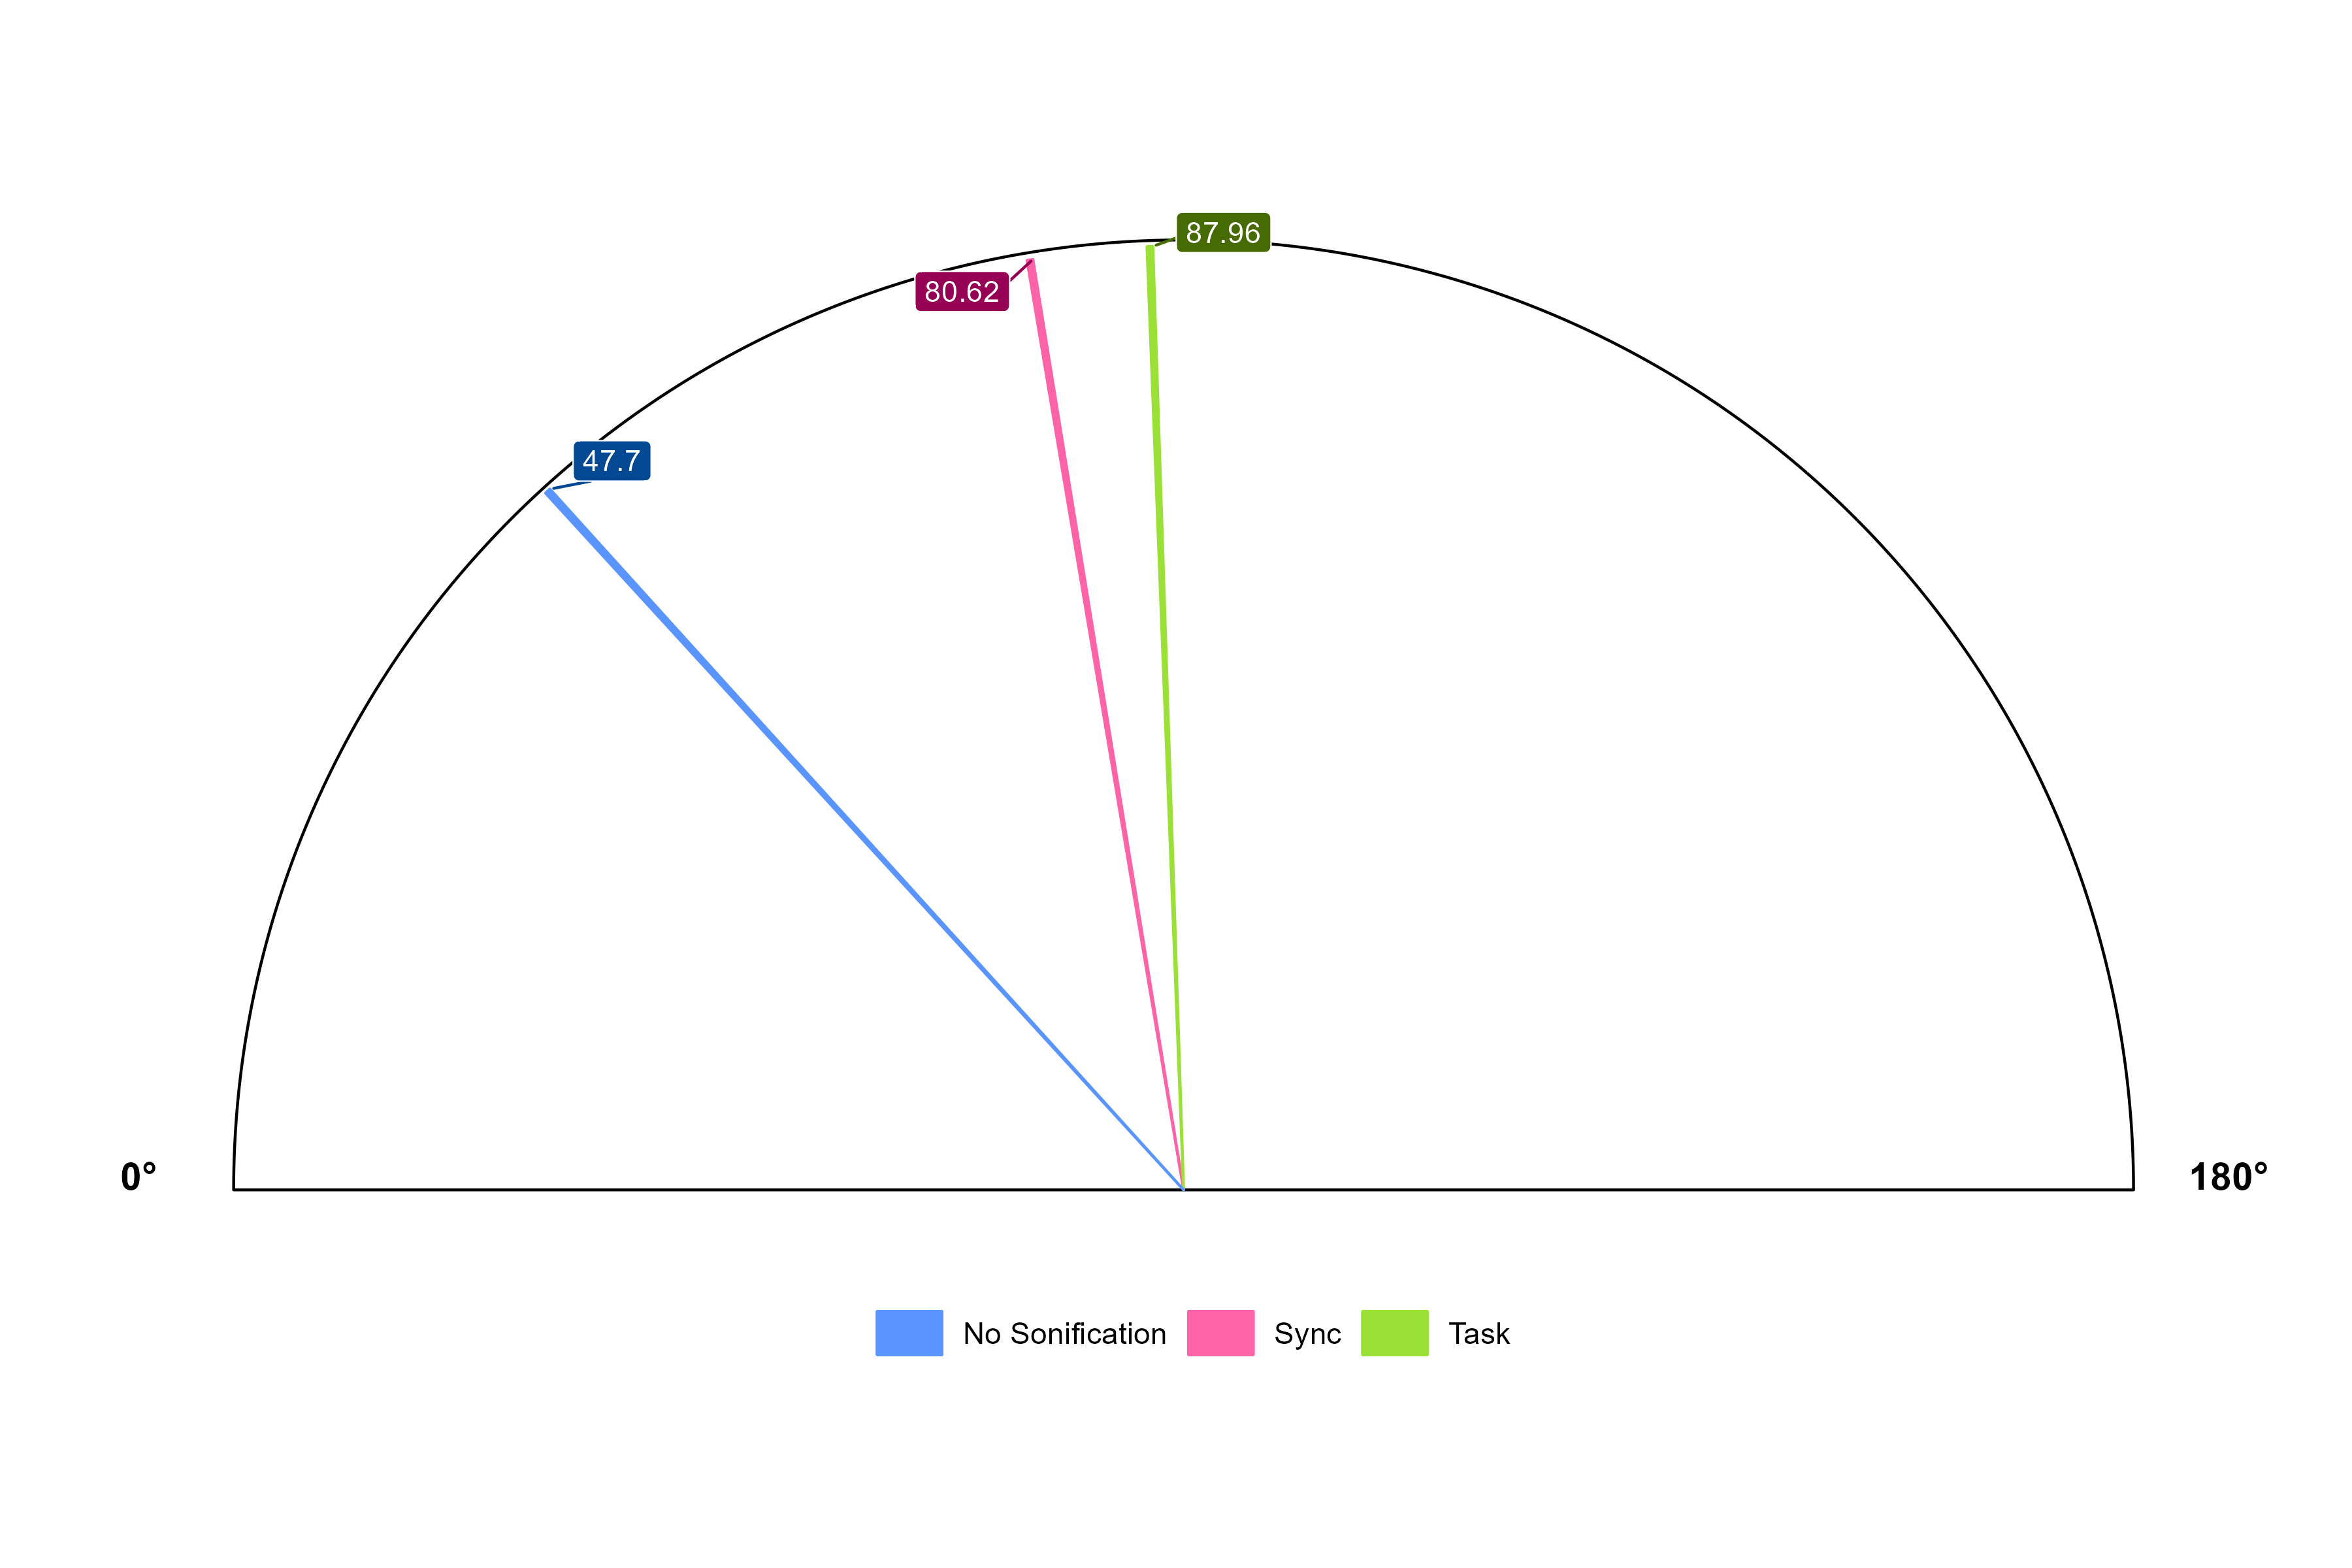
\includegraphics[width=1\linewidth]{figures/mean_condition_phase_angles_mean_sd} 

}

\caption{Plot of mean absolute instantaneous phase angles of experimental conditions with the length of the needles representing the standard deviation as a percentage of 90 degrees. No Sonification condition mean phase angle =  8.861 (sd =  0.067 ) degrees, task sonification condition mean phase angle =  14.211 (sd =  0.216 ) degrees, sync sonification condition mean phase angle =  8.749 (sd =  0.075 ) degrees.}\label{fig:mean-instantaneous-phase-angle-circular-plot}
\end{figure}

\hypertarget{dynamic-time-warping}{%
\subsubsection{Dynamic Time Warping}\label{dynamic-time-warping}}

Dynamic Time Warping (DTW) is a method used to compare two sequences of data, typically when the sequences are of unequal length or have non-linear variations. DTW works by finding the optimal alignment between the two sequences by stretching or compressing one sequence so that the difference between the two sequences is minimized. This alignment is represented by a mapping function that indicates the relationship between the two sequences at each point in time. DTW has found applications in a wide range of fields, including speech recognition, music analysis, and activity recognition, among others. In the context of your experiment, DTW can be used to compare the trajectories of the two sleds and assess the level of synchrony between them over time, allowing for a more detailed analysis of the movement patterns. For the analysis, data were decimated, resulting in a sample rate of 30 Hz which reduced the computation time significantly and comparisons between several full-rate and downsampled DTW analyses resulted in comparable normalized path distances.

\begin{figure}[h]

{\centering 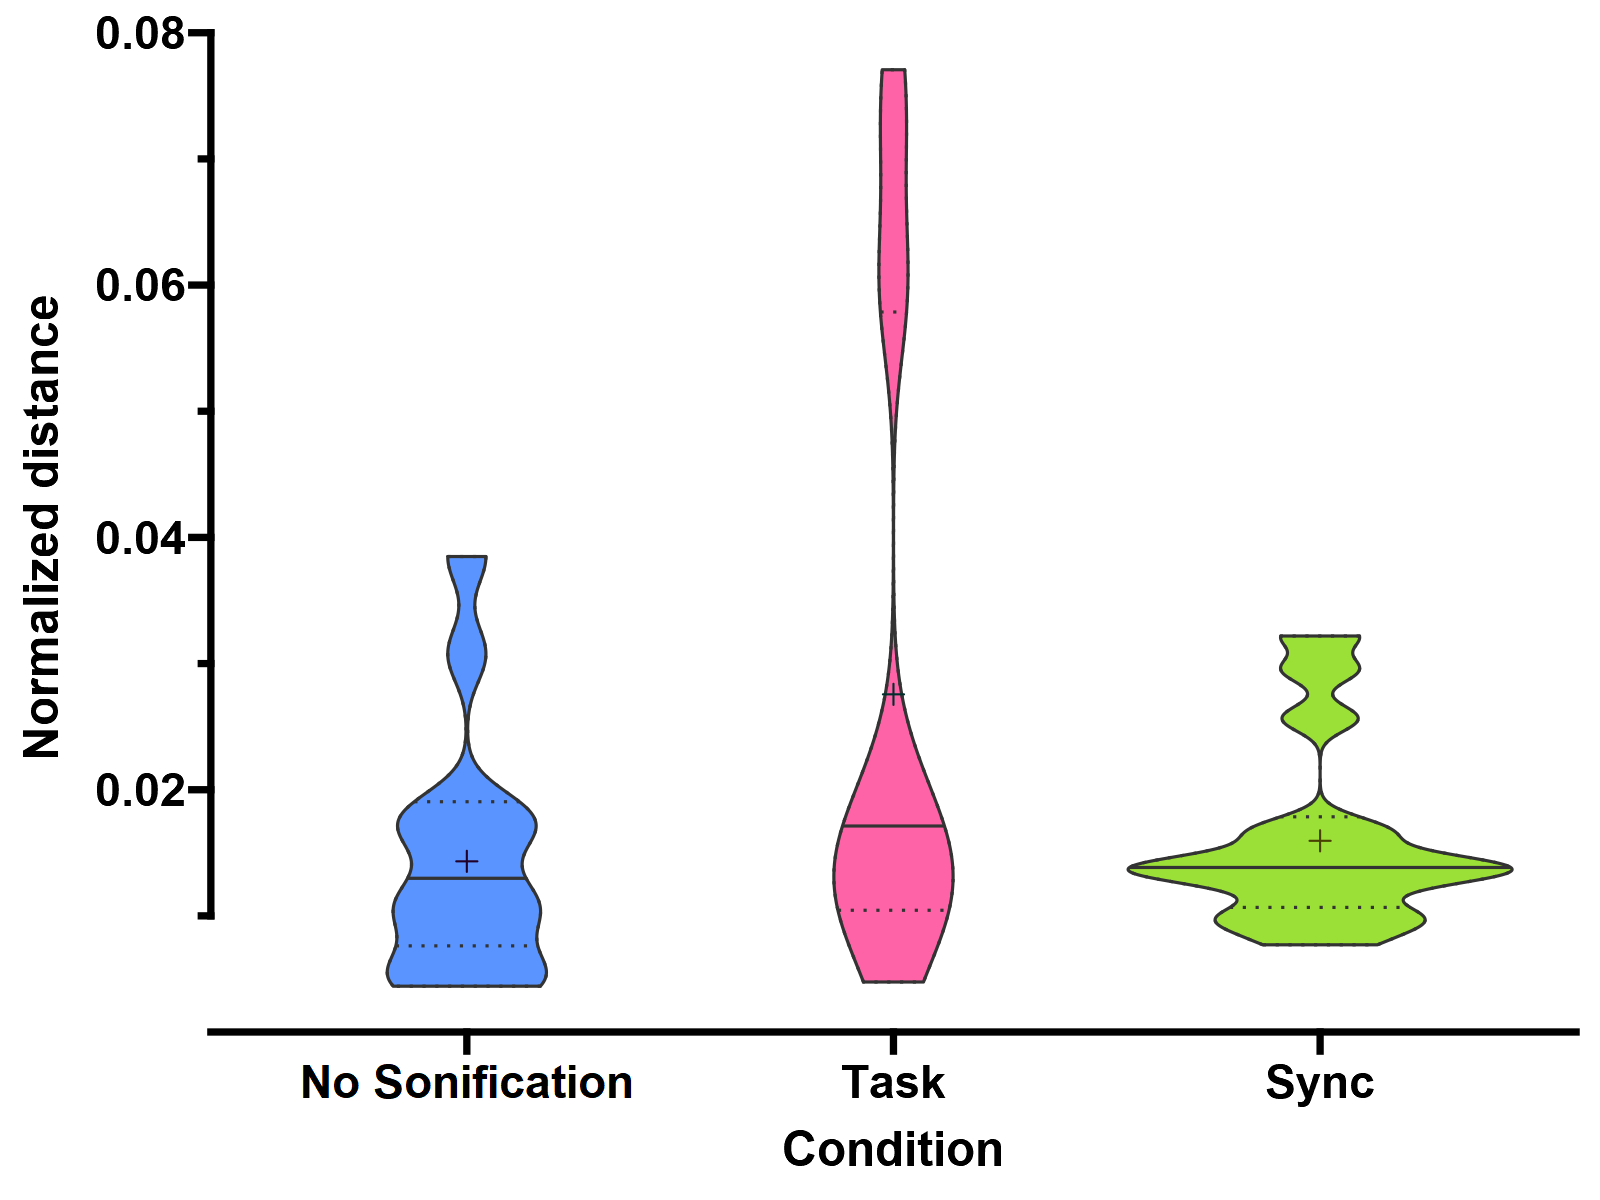
\includegraphics[width=1\linewidth]{figures/dtw_summary} 

}

\caption{Distribution density plot of normalized dynamic time warp path distance between paired trajectories by condition. The mean normalized distance is shown as a point (+), the 20th and 80th percentiles are shown as dashed lines and the 50th percentile is shown as a solid line. No Sonification condition normalized distance mean  =  0.014 (sd =  0.01 ) degrees, task sonification condition normalized distance mean =  0.028 (sd =  0.025 ) degrees, sync sonification condition normalized distance mean =  0.016 (sd =  0.007 ) degrees.}(\#fig:dtw-plot, )
\end{figure}

\hypertarget{learning}{%
\subsection{Learning}\label{learning}}

{[}optional{]} include simple analysis of mean / sd by trial

\hypertarget{results}{%
\section{Results}\label{results}}

\hypertarget{spatial-difference}{%
\subsection{Spatial Difference}\label{spatial-difference}}

\hypertarget{instantaneous-phase-angle}{%
\subsection{Instantaneous Phase Angle}\label{instantaneous-phase-angle}}

The results showed that the mean angle difference
was 8.861° ± 0.067° (SD) for the no sonification condition,
14.211° ± 0.216° (SD) for the task condition, and
8.749° ± 0.075° (SD) for the sync condition. (Figure \ref{fig:mean-instantaneous-phase-angle-circular-plot}).

\hypertarget{dynamic-time-warping-1}{%
\subsection{Dynamic Time Warping}\label{dynamic-time-warping-1}}

\hypertarget{discussion}{%
\section{Discussion}\label{discussion}}

{[}Explain{]}

Although we could not completely isolate the joint action representations, partially due to sound created from the movement of the sleds, our sonification primes attention towards either self-other monitoring by sonification of both sled positions independently, or joint outcome by sonification of the positions of each sled relative to the other.

How might our task be affected by musical training? ``Successful music performance requires that musicians monitor the auditory consequences of their actions. Years of training on an instrument lead to strong associations between a given movement or set of movements and a given auditory outcome.'' (Loehr et al., 2013)

ML model applications in this project?
Other analysis methods yielded similar results, brief explanation
Could consider another sonification to compare to: besides no sonification / dealing with spatial audio, could also have a regular beep to mark when they should be at the ends, or even a constant range representing where they should be (i.e.~directing their movements with the sound rather than sonification of their movement, this could be another type of control and represent some more traditional methods)
Loudness and brightness may be better choices for modulation targets than pitch changes: \autocite{mcdermottMusicalIntervalsRelative2010}

Mention the marker placement as being problematic. Also the number of reference markers\ldots also that we wanted to use headphones\ldots{}
Additionally, we could have had start and end checkpoints where it could be used to segment the data into sub-trials or maybe even make participants stop and wait (but that ruins flow)

Mention analysis of learning effect, not enough data here, too many invalid trials, but would be interesting to see if participants ``learn'' the sonification schemes

• How does our task compare to e.g.~Loehr et al.~piano duet task?
• What can and can't our task reveal?
o Can't say that only one of the participants makes a mistake, since the goal is to in sync with each other, without a general ``tempo'' to follow
• Individual representations vs joint outcome representations?
o Often can't mirror the other person exactly

if someone wanted to reproduce we can talk about things like the height of the track, the width of the base making it less comfortable, the range in participant music experience, also the fact that the mocap lab is small and there were problems making camera trakcing more difficult.

and of course all the stuff about different sonification options and testing ranges of values to see what works, and whole new strategies we haven't thought of using headphones to stop the track noise which subjects noted they used\ldots{}
and of course we can talk about that in relation to the results, lack of results, why we might be seeing the data we see,

and especially that we actually managed to create a low-latency method for sonification of /arbitrary/ data, and we used it for an expensive mocap setup but this could be applied to outputs from machine learning models (i.e.~webcam object tracking) or even other low-cost hardware like wiimotes or something

we also don't use pure sine tones, so the more complex tones might make it more difficult to distinguish.,..we could try also octaves, perhaps it is easier to distinguish for nonmusicians.
Maybe we can add more dimensions

{[}optional{]} include simple analysis of mean / sd by trial in analyses

Applications
Movement sonification + joint action is useful for training sports, e.g.~rowing, but also track relay, where two runners try to optimize the timing when passing the baton

\begin{figure}[h]

{\centering 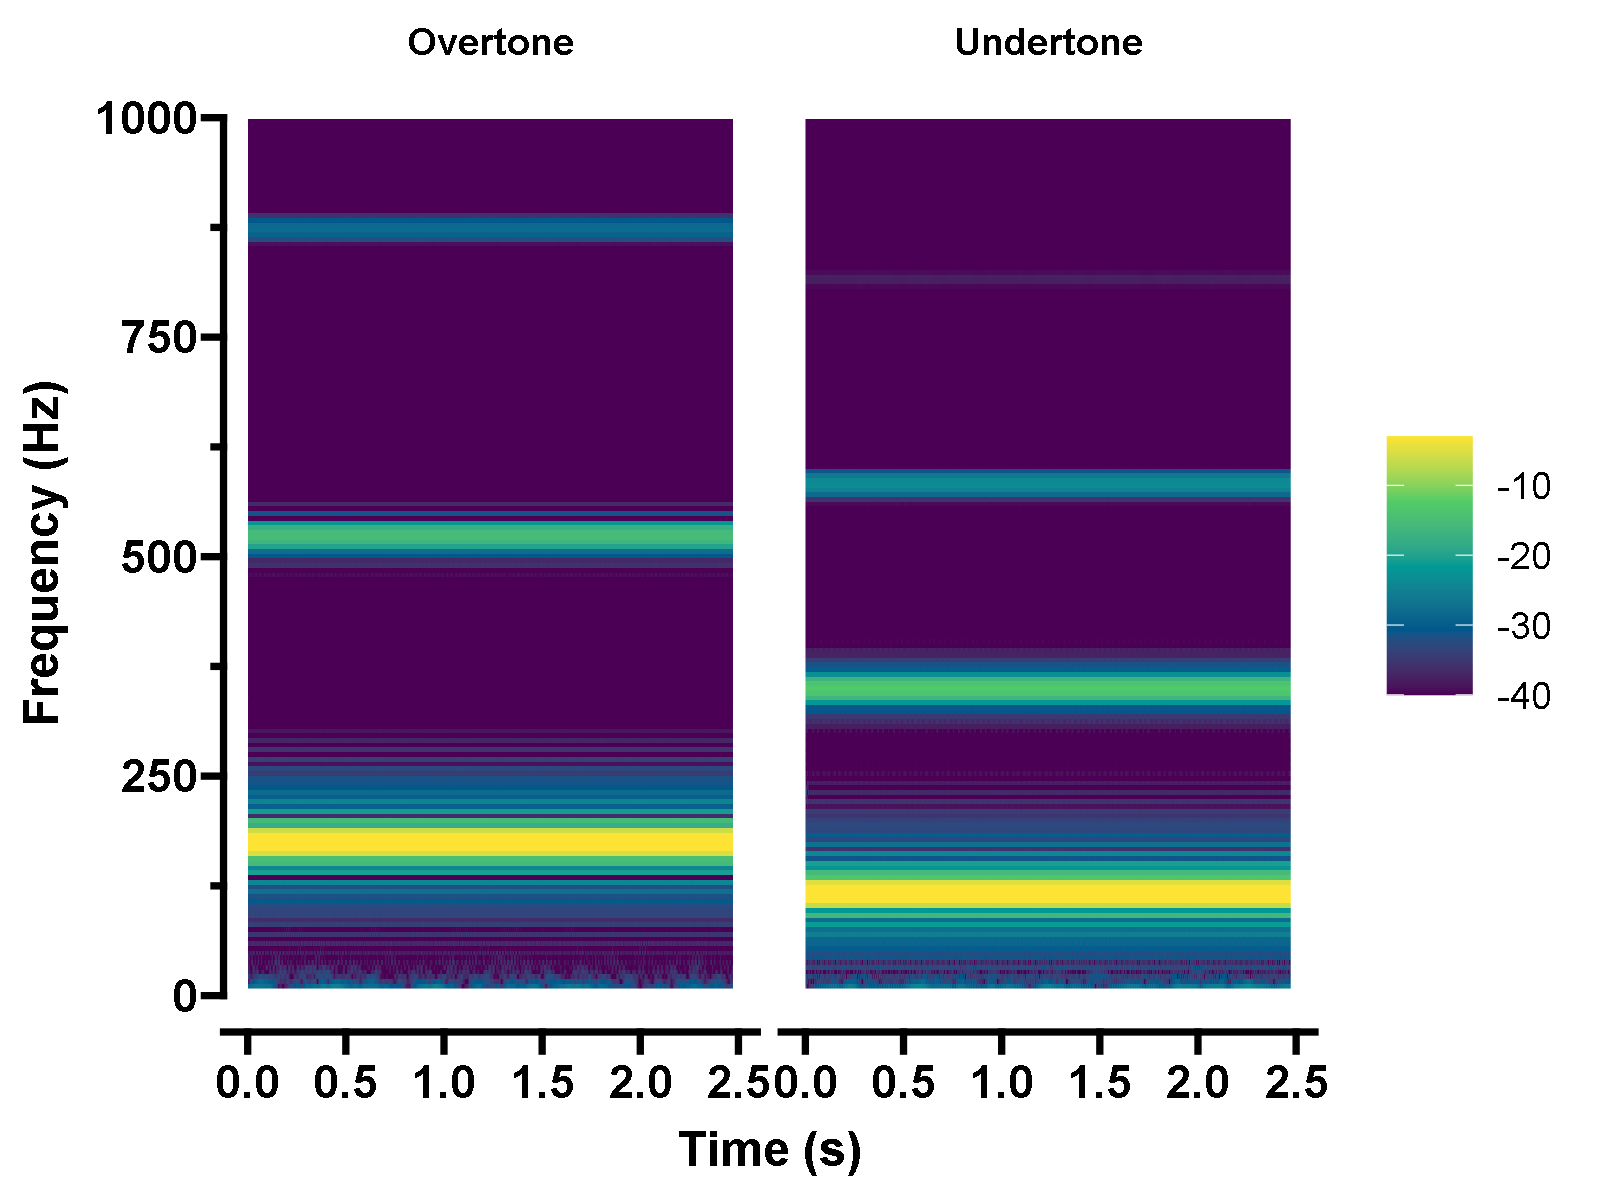
\includegraphics[width=1\linewidth]{figures/spec_tones} 

}

\caption{Spectral analysis of the two base frequency audio files}\label{fig:stimuli-spectra}
\end{figure}
\balance
\clearpage


\printbibliography[title=References,heading=bibintoc]

\end{document}
